% 1) pdflatex main
% 2) makeindex main.idx -s StyleInd.ist
% 3) biber main
% 4) pdflatex main x 2
\documentclass[11pt,fleqn]{book} % Default font size and left-justified equations
\usepackage[top=3cm,bottom=3cm,left=3.2cm,right=3.2cm,headsep=10pt,a4paper]{geometry} % Page margins
\usepackage{xcolor} % Required for specifying colors by name
\definecolor{ocre}{RGB}{243,102,25} % Define the orange color used for highlighting throughout the book
% Font Settings
\usepackage{avant} % Use the Avantgarde font for headings
\usepackage{times} % Use the Times font for headings
\usepackage{mathptmx} % Use the Adobe Times Roman as the default text font together with math symbols from the Sym­bol, Chancery and Com­puter Modern fonts

\usepackage{microtype} % Slightly tweak font spacing for aesthetics
                                                                                                                                                                                                                                                                                                                                                                                                     \usepackage[utf8]{inputenc} % Required for including letters with accents
\usepackage[T1]{fontenc} % Use 8-bit encoding that has 256 glyphs

\usepackage{amsmath,amssymb,amsfonts,latexsym}
\usepackage{latexsym}
\usepackage{amsmath}
\usepackage{amsfonts}
\usepackage[spanish]{babel}
\usepackage{mathrsfs}
\usepackage{psfrag}
\usepackage{graphicx}
\usepackage{amssymb}
\usepackage{multirow}
\usepackage{rotating}
\usepackage{enumerate}

\usepackage{cancel}

\usepackage{subfig}%PARA LAS FIGURAS MULTIPLES
\usepackage{multicol}


%\usepackage{enumitem}
%\usepackage[version=3]{mhchem}


\usepackage[spanish]{babel}

\spanishdecimal{.} %PARA EL PUNTO DECIMAL

% Bibliography
\usepackage[style=alphabetic,sorting=nyt,sortcites=true,autopunct=true,babel=hyphen,hyperref=true,abbreviate=false,backref=true,backend=biber]{biblatex}
\addbibresource{bibliography.bib} % BibTeX bibliography file
\defbibheading{bibempty}{}

% Index
\usepackage{calc} % For simpler calculation - used for spacing the index letter headings correctly
\usepackage{makeidx} % Required to make an index
\makeindex % Tells LaTeX to create the files required for indexing
%----------------------------------------------------------------------------------------

%----------------------------------------------------------------------------------------
%	VARIOUS REQUIRED PACKAGES
%----------------------------------------------------------------------------------------

\usepackage{titlesec} % Allows customization of titles

\usepackage{graphicx} % Required for including pictures
\graphicspath{{Pictures/}} % Specifies the directory where pictures are stored

\usepackage{lipsum} % Inserts dummy text

\usepackage{tikz} % Required for drawing custom shapes

\usepackage[spanish]{babel} % english language/hyphenation

\usepackage{enumitem} % Customize lists
\setlist{nolistsep} % Reduce spacing between bullet points and numbered lists

\usepackage{booktabs} % Required for nicer horizontal rules in tables

\usepackage{eso-pic} % Required for specifying an image background in the title page

%----------------------------------------------------------------------------------------
%	MAIN TABLE OF CONTENTS
%----------------------------------------------------------------------------------------

\usepackage{titletoc} % Required for manipulating the table of contents

\contentsmargin{0cm} % Removes the default margin
% Chapter text styling
\titlecontents{chapter}[1.25cm] % Indentation
{\addvspace{15pt}\large\sffamily\bfseries} % Spacing and font options for chapters
{\color{ocre!60}\contentslabel[\Large\thecontentslabel]{1.25cm}\color{ocre}} % Chapter number
{}
{\color{ocre!90}\normalsize\sffamily\bfseries\;\titlerule*[.5pc]{.}\;\thecontentspage} % Page number
% Section text styling
\titlecontents{section}[1.25cm] % Indentation
{\addvspace{5pt}\sffamily\bfseries} % Spacing and font options for sections
{\contentslabel[\thecontentslabel]{1.25cm}} % Section number
{}
{\sffamily\hfill\color{black}\thecontentspage} % Page number
[]
% Subsection text styling
\titlecontents{subsection}[1.25cm] % Indentation
{\addvspace{1pt}\sffamily\small} % Spacing and font options for subsections
{\contentslabel[\thecontentslabel]{1.25cm}} % Subsection number
{}
{\sffamily\;\titlerule*[.5pc]{.}\;\thecontentspage} % Page number
[]

%----------------------------------------------------------------------------------------
%	MINI TABLE OF CONTENTS IN CHAPTER HEADS
%----------------------------------------------------------------------------------------

% Section text styling
\titlecontents{lsection}[0em] % Indendating
{\footnotesize\sffamily} % Font settings
{}
{}
{}

% Subsection text styling
\titlecontents{lsubsection}[.5em] % Indentation
{\normalfont\footnotesize\sffamily} % Font settings
{}
{}
{}

%----------------------------------------------------------------------------------------
%	PAGE HEADERS
%----------------------------------------------------------------------------------------

\usepackage{fancyhdr} % Required for header and footer configuration

\pagestyle{fancy}
\renewcommand{\chaptermark}[1]{\markboth{\sffamily\normalsize\bfseries #1}{}} % Chapter text font settings
\renewcommand{\sectionmark}[1]{\markright{\sffamily\normalsize\thesection\hspace{5pt}#1}{}} % Section text font settings
\fancyhf{} \fancyhead[LE,RO]{\sffamily\normalsize\thepage} % Font setting for the page number in the header
\fancyhead[LO]{\rightmark} % Print the nearest section name on the left side of odd pages
\fancyhead[RE]{\leftmark} % Print the current chapter name on the right side of even pages
\renewcommand{\headrulewidth}{0.5pt} % Width of the rule under the header
\addtolength{\headheight}{2.5pt} % Increase the spacing around the header slightly
\renewcommand{\footrulewidth}{0pt} % Removes the rule in the footer
\fancypagestyle{plain}{\fancyhead{}\renewcommand{\headrulewidth}{0pt}} % Style for when a plain pagestyle is specified

% Removes the header from odd empty pages at the end of chapters
\makeatletter
\renewcommand{\cleardoublepage}{
\clearpage\ifodd\c@page\else
\hbox{}
\vspace*{\fill}
\thispagestyle{empty}
\newpage
\fi}

%----------------------------------------------------------------------------------------
%	THEOREM STYLES
%----------------------------------------------------------------------------------------

\usepackage{amsmath,amsfonts,amssymb,amsthm} % For including math equations, theorems, symbols, etc

\newcommand{\intoo}[2]{\mathopen{]}#1\,;#2\mathclose{[}}
\newcommand{\ud}{\mathop{\mathrm{{}d}}\mathopen{}}
\newcommand{\intff}[2]{\mathopen{[}#1\,;#2\mathclose{]}}
\newtheorem{notation}{Notaci\'on}[chapter]




%%%%%%%%%%%%%%%%%%%%%%%%%%%%%%%%%%%%%%%%%%%%%%%%%%%%%%%%%%%%%%%%%%%%%%%%%%%
%%%%%%%%%%%%%%%%%%%% dedicated to boxed/framed environements %%%%%%%%%%%%%%
%%%%%%%%%%%%%%%%%%%%%%%%%%%%%%%%%%%%%%%%%%%%%%%%%%%%%%%%%%%%%%%%%%%%%%%%%%%
\newtheoremstyle{ocrenumbox}% % Theorem style name
{0pt}% Space above
{0pt}% Space below
{\normalfont}% % Body font
{}% Indent amount
{\small\bf\sffamily\color{ocre}}% % Theorem head font
{\;}% Punctuation after theorem head
{0.25em}% Space after theorem head
{\small\sffamily\color{ocre}\thmname{#1}\nobreakspace\thmnumber{\@ifnotempty{#1}{}\@upn{#2}}% Theorem text (e.g., Theorem 2.1)
\thmnote{\nobreakspace\the\thm@notefont\sffamily\bfseries\color{black}---\nobreakspace#3.}} % Optional theorem note
\renewcommand{\qedsymbol}{$\blacksquare$}% Optional qed square

\newtheoremstyle{blacknumex}% Theorem style name
{5pt}% Space above
{5pt}% Space below
{\normalfont}% Body font
{} % Indent amount
{\small\bf\sffamily}% Theorem head font
{\;}% Punctuation after theorem head
{0.25em}% Space after theorem head
{\small\sffamily{\tiny\ensuremath{\blacksquare}}\nobreakspace\thmname{#1}\nobreakspace\thmnumber{\@ifnotempty{#1}{}\@upn{#2}}% Theorem text (e.g., Theorem 2.1)
\thmnote{\nobreakspace\the\thm@notefont\sffamily\bfseries---\nobreakspace#3.}}% Optional theorem note

\newtheoremstyle{blacknumbox} % Theorem style name
{0pt}% Space above
{0pt}% Space below
{\normalfont}% Body font
{}% Indent amount
{\small\bf\sffamily}% Theorem head font
{\;}% Punctuation after theorem head
{0.25em}% Space after theorem head
{\small\sffamily\thmname{#1}\nobreakspace\thmnumber{\@ifnotempty{#1}{}\@upn{#2}}% Theorem text (e.g., Theorem 2.1)
\thmnote{\nobreakspace\the\thm@notefont\sffamily\bfseries---\nobreakspace#3.}}% Optional theorem note

%%%%%%%%%%%%%%%%%%%%%%%%%%%%%%%%%%%%%%%%%%%%%%%%%%%%%%%%%%%%%%%%%%%%%%%%%%%
%%%%%%%%%%%%% dedicated to non-boxed/non-framed environements %%%%%%%%%%%%%
%%%%%%%%%%%%%%%%%%%%%%%%%%%%%%%%%%%%%%%%%%%%%%%%%%%%%%%%%%%%%%%%%%%%%%%%%%%
\newtheoremstyle{ocrenum}% % Theorem style name
{5pt}% Space above
{5pt}% Space below
{\normalfont}% % Body font
{}% Indent amount
{\small\bf\sffamily\color{ocre}}% % Theorem head font
{\;}% Punctuation after theorem head
{0.25em}% Space after theorem head
{\small\sffamily\color{ocre}\thmname{#1}\nobreakspace\thmnumber{\@ifnotempty{#1}{}\@upn{#2}}% Theorem text (e.g., Theorem 2.1)
\thmnote{\nobreakspace\the\thm@notefont\sffamily\bfseries\color{black}---\nobreakspace#3.}} % Optional theorem note
\renewcommand{\qedsymbol}{$\blacksquare$}% Optional qed square
\makeatother

% Defines the theorem text style for each type of theorem to one of the three styles above
\newcounter{dummy}
\numberwithin{dummy}{section}
\theoremstyle{ocrenumbox}
\newtheorem{theoremeT}[dummy]{Teorema}
\newtheorem{LemaT}[dummy]{Lema}
\newtheorem{problem}{Problema}[chapter]
\newtheorem{exerciseT}{Ejercicio}[chapter]
\theoremstyle{blacknumex}
\newtheorem{exampleT}{Ejemplo}[chapter]
\theoremstyle{blacknumbox}
\newtheorem{vocabulary}{Vocabulario}[chapter]
\newtheorem{definitionT}{Definici\'on}[section]
\newtheorem{corollaryT}[dummy]{Corolario}
\theoremstyle{ocrenum}
\newtheorem{proposition}[dummy]{Proposici\'on}
\newtheorem{obsT}{Observaci\'on}[chapter]

%----------------------------------------------------------------------------------------
%	DEFINITION OF COLORED BOXES
%----------------------------------------------------------------------------------------

\RequirePackage[framemethod=default]{mdframed} % Required for creating the theorem, definition, exercise and corollary boxes

% Theorem box
\newmdenv[skipabove=7pt,
skipbelow=7pt,
backgroundcolor=black!5,
linecolor=ocre,
innerleftmargin=5pt,
innerrightmargin=5pt,
innertopmargin=5pt,
leftmargin=0cm,
rightmargin=0cm,
innerbottommargin=5pt]{tBox}

% Exercise box
\newmdenv[skipabove=7pt,
skipbelow=7pt,
rightline=false,
leftline=true,
topline=false,
bottomline=false,
backgroundcolor=ocre!10,
linecolor=ocre,
innerleftmargin=5pt,
innerrightmargin=5pt,
innertopmargin=5pt,
innerbottommargin=5pt,
leftmargin=0cm,
rightmargin=0cm,
linewidth=4pt]{eBox}

% Definition box
\newmdenv[skipabove=7pt,
skipbelow=7pt,
rightline=false,
leftline=true,
topline=false,
bottomline=false,
linecolor=ocre,
innerleftmargin=5pt,
innerrightmargin=5pt,
innertopmargin=0pt,
leftmargin=0cm,
rightmargin=0cm,
linewidth=4pt,
innerbottommargin=0pt]{dBox}

% Corollary box
\newmdenv[skipabove=7pt,
skipbelow=7pt,
rightline=false,
leftline=true,
topline=false,
bottomline=false,
linecolor=gray,
backgroundcolor=black!5,
innerleftmargin=5pt,
innerrightmargin=5pt,
innertopmargin=5pt,
leftmargin=0cm,
rightmargin=0cm,
linewidth=4pt,
innerbottommargin=5pt]{cBox}



% Observation box
\newmdenv[skipabove=7pt,
skipbelow=7pt,
rightline=false,
leftline=false,
topline=false,
bottomline=false,
backgroundcolor=ocre!10,
linecolor=ocre,
innerleftmargin=5pt,
innerrightmargin=5pt,
innertopmargin=5pt,
innerbottommargin=5pt,
leftmargin=0cm,
rightmargin=0cm,
linewidth=4pt]{oBox}

% X Box
\newmdenv[skipabove=7pt,
skipbelow=7pt,
backgroundcolor=ocre!10, %black!5,
linecolor=ocre,
innerleftmargin=5pt,
innerrightmargin=5pt,
innertopmargin=5pt,
leftmargin=0cm,
rightmargin=0cm,
innerbottommargin=5pt]{xBox}

%Caja simple
\newenvironment{xbox}[1][\unskip]{%
\begin{xBox}
\textbf{\sffamily\color{ocre} #1\\}
%\textbf{#1\\}
}
{\end{xBox}}

% Creates an environment for each type of theorem and assigns it a theorem text style from the "Theorem Styles" section above and a colored box from above
\newenvironment{theorem}{\begin{tBox}\begin{theoremeT}}{\end{theoremeT}\end{tBox}}
\newenvironment{Lema}{\begin{tBox}\begin{LemaT}}{\end{LemaT}\end{tBox}}
\newenvironment{exercise}{\begin{eBox}\begin{exerciseT}}{\hfill{\color{ocre}\tiny\ensuremath{\blacksquare}}\end{exerciseT}\end{eBox}}
\newenvironment{definition}{\begin{dBox}\begin{definitionT}}{\end{definitionT}\end{dBox}}
\newenvironment{example}{\begin{exampleT}}{\hfill{\tiny\ensuremath{\blacksquare}}\end{exampleT}}
\newenvironment{corollary}{\begin{cBox}\begin{corollaryT}}{\end{corollaryT}\end{cBox}}

\newenvironment{obs}{\begin{oBox}\begin{obsT}}{\hfill{\color{ocre}\tiny}\end{obsT}\end{oBox}}


%----------------------------------------------------------------------------------------
%	REMARK OBSERVATION
%----------------------------------------------------------------------------------------
%
%\newenvironment{obs}{
%\begin{center}
%\begin{tabular}{p{10cm}}
%{\color{ocre} \textbf{Observaci\'on}}:
%\end{tabular}
%\end{center}
%}

%----------------------------------------------------------------------------------------
%	SECTION NUMBERING IN THE MARGIN
%----------------------------------------------------------------------------------------

\makeatletter
\renewcommand{\@seccntformat}[1]{\llap{\textcolor{ocre}{\csname the#1\endcsname}\hspace{1em}}}
\renewcommand{\section}{\@startsection{section}{1}{\z@}
{-4ex \@plus -1ex \@minus -.4ex}
{1ex \@plus.2ex }
{\normalfont\large\sffamily\bfseries}}
\renewcommand{\subsection}{\@startsection {subsection}{2}{\z@}
{-3ex \@plus -0.1ex \@minus -.4ex}
{0.5ex \@plus.2ex }
{\normalfont\sffamily\bfseries}}
\renewcommand{\subsubsection}{\@startsection {subsubsection}{3}{\z@}
{-2ex \@plus -0.1ex \@minus -.2ex}
{0.2ex \@plus.2ex }
{\normalfont\small\sffamily\bfseries}}
\renewcommand\paragraph{\@startsection{paragraph}{4}{\z@}
{-2ex \@plus-.2ex \@minus .2ex}
{0.1ex}
{\normalfont\small\sffamily\bfseries}}

%----------------------------------------------------------------------------------------
%	CHAPTER HEADINGS
%----------------------------------------------------------------------------------------

\newcommand{\thechapterimage}{}
\newcommand{\chapterimage}[1]{\renewcommand{\thechapterimage}{#1}}
\def\thechapter{\arabic{chapter}}
\def\@makechapterhead#1{
\thispagestyle{empty}
{\centering \normalfont\sffamily
\ifnum \c@secnumdepth >\m@ne
\if@mainmatter
\startcontents
\begin{tikzpicture}[remember picture,overlay]
\node at (current page.north west)
{\begin{tikzpicture}[remember picture,overlay]

\node[anchor=north west,inner sep=0pt] at (0,0) {\includegraphics[width=\paperwidth]{\thechapterimage}};

%Commenting the 3 lines below removes the small contents box in the chapter heading
\draw[fill=white,opacity=.6] (1cm,0) rectangle (8cm,-7cm);
\node[anchor=north west] at (1cm,.25cm) {\parbox[t][8cm][t]{6.5cm}{\huge\bfseries\flushleft \printcontents{l}{1}{\setcounter{tocdepth}{2}}}};

\draw[anchor=west] (5cm,-9cm) node [rounded corners=25pt,fill=white,fill opacity=.6,text opacity=1,draw=ocre,draw opacity=1,line width=2pt,inner sep=15pt]{\huge\sffamily\bfseries\textcolor{black}{\thechapter\ ---\ #1\vphantom{plPQq}\makebox[22cm]{}}};
\end{tikzpicture}};
\end{tikzpicture}}\par\vspace*{230\p@}
\fi
\fi
}
\def\@makeschapterhead#1{
\thispagestyle{empty}
{\centering \normalfont\sffamily
\ifnum \c@secnumdepth >\m@ne
\if@mainmatter
\startcontents
\begin{tikzpicture}[remember picture,overlay]
\node at (current page.north west)
{\begin{tikzpicture}[remember picture,overlay]
\node[anchor=north west] at (-4pt,4pt) {\includegraphics[width=\paperwidth]{\thechapterimage}};
\draw[anchor=west] (5cm,-9cm) node [rounded corners=25pt,fill=white,opacity=.7,inner sep=15.5pt]{\huge\sffamily\bfseries\textcolor{black}{\vphantom{plPQq}\makebox[22cm]{}}};
\draw[anchor=west] (5cm,-9cm) node [rounded corners=25pt,draw=ocre,line width=2pt,inner sep=15pt]{\huge\sffamily\bfseries\textcolor{black}{#1\vphantom{plPQq}\makebox[22cm]{}}};
\end{tikzpicture}};
\end{tikzpicture}}\par\vspace*{230\p@}
\fi
\fi
}
\makeatother
 % Insert the commands.tex file which contains the majority of the structure behind the template


%DEFINICION DE LA CONSTANTE ELECTRICA
\newcommand{\ke}{ \frac{1}{4\pi \varepsilon_0 }}


%DEFINICION DEL VECTOR RADIAL UNITARIO PRIMADO
\newcommand{\rup}{ \mathbf{\hat{r}}\textsc{\textbf{'}} }






\begin{document}


%----------------------------------------------------------------------------------------
%	TITLE PAGE
%----------------------------------------------------------------------------------------
%\begingroup
%\thispagestyle{empty}
%\AddToShipoutPicture*{\put(6,5){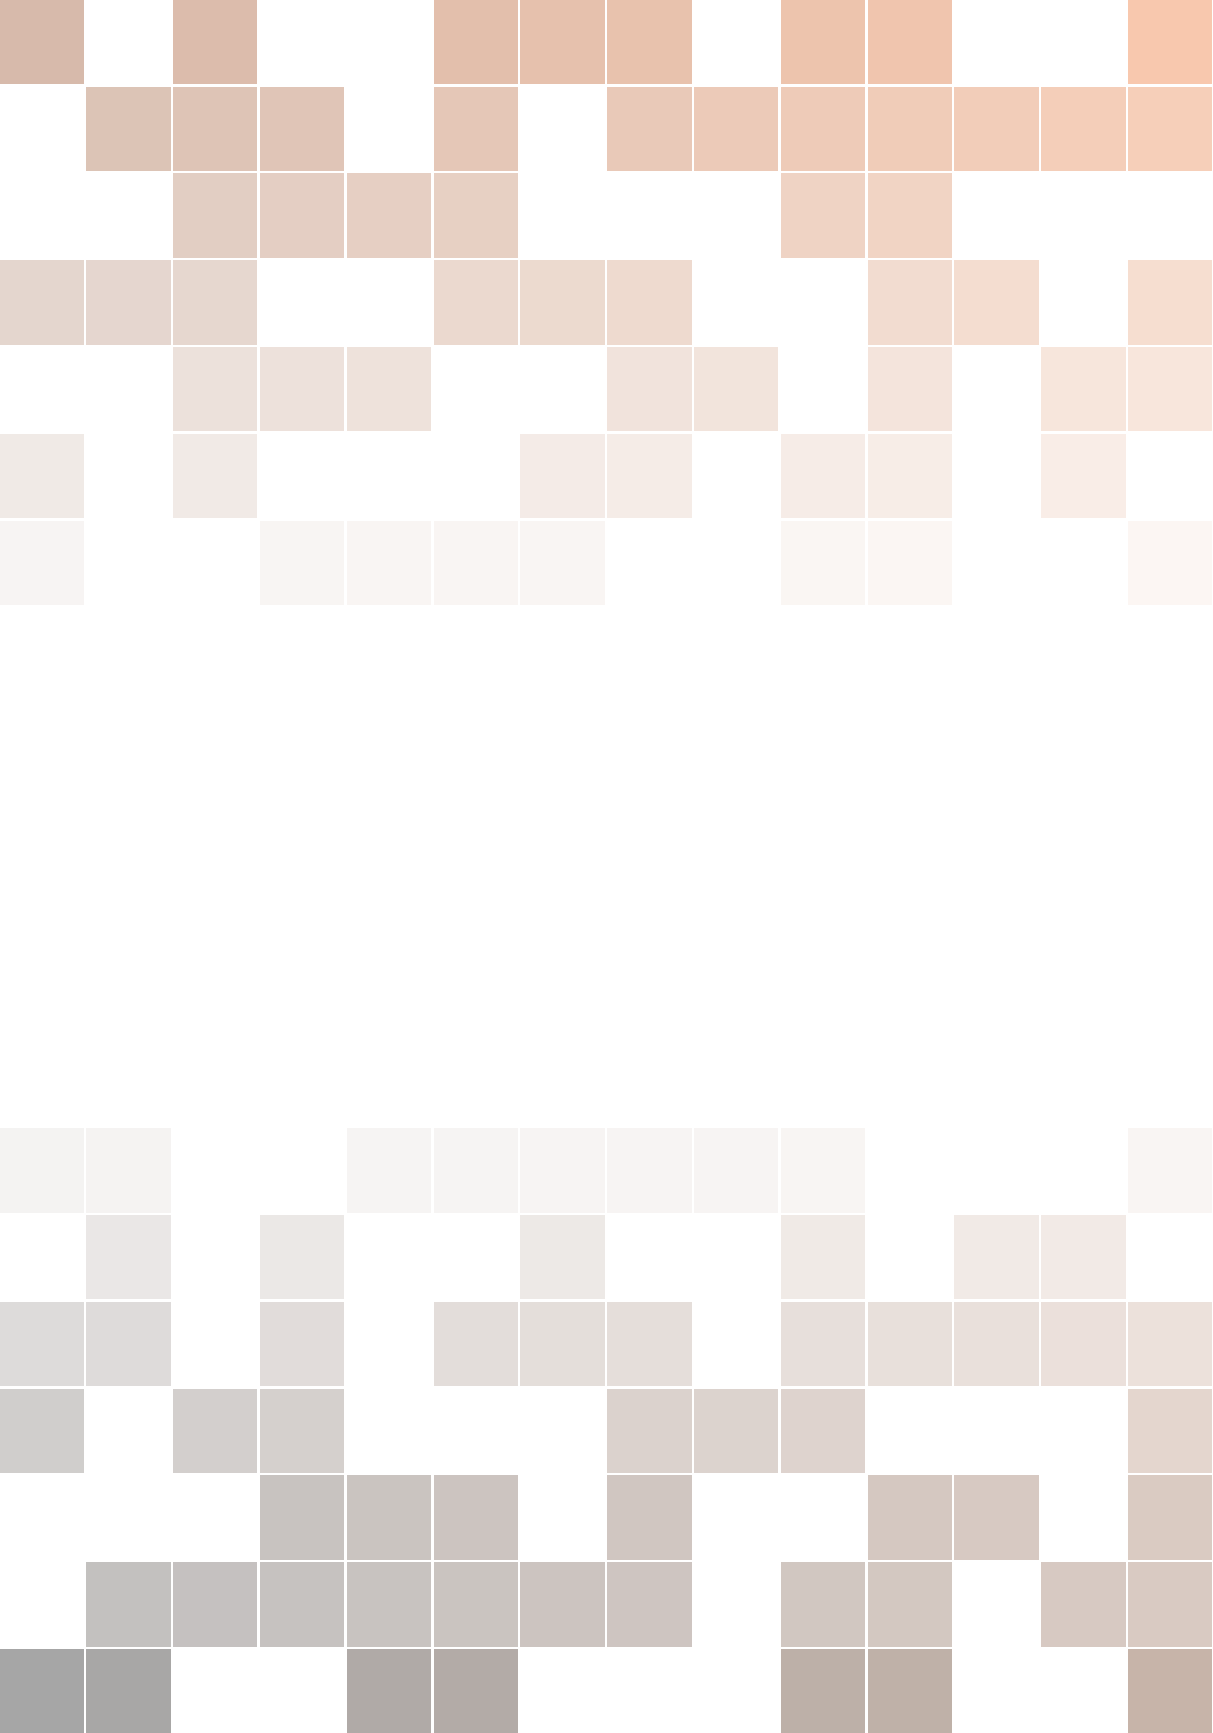
\includegraphics[scale=1]{background}}} % Image background
%\centering
%\vspace*{9cm}
%\par\normalfont\fontsize{35}{35}\sffamily\selectfont
%Mec\'anica Cl\'asica\par % Book title
%\vspace*{1cm}
%{\Huge Autores}\par % Author name
%\endgroup

%----------------------------------------------------------------------------------------
%	TABLE OF CONTENTS
%----------------------------------------------------------------------------------------
\chapterimage{Electro1} % Table of contents heading image
\pagestyle{empty} % No headers
\tableofcontents % Print the table of contents itself
\cleardoublepage % Forces the first chapter to start on an odd page so it's on the right

\pagestyle{fancy} % Print headers again


\chapter{Ondas electromagn\'eticas planas}
\section{En el vac\'io: velocidades de fase y transporte energ\'ia. Transversalidad y polarizaci\'on.}

Se sabe que cualquier soluci\'on de las ecuaciones de Maxwell que satisfagan ciertas condiciones de frontera dadas por campos electromagn\'eticos producidos por densidades de
carga y corriente adecuadas, da como resultado una onda electromagn\'etica. Pero en la pr\'actica no es conveniente resolver las ecuaciones de Maxwell indiscriminadamente para
obtener el comportamiento de dichas ondas.\\
Para ello es mejor resolver las ecuaci\'on de onda propuesta en el cap\'itulo anterior,
\begin{equation}\label{EcOndaCom}
 \nabla^2 \psi-\sigma\mu\frac{\partial \psi}{\partial t}-\epsilon\mu\frac{\partial^2 \psi}{\partial t^2}=0,
\end{equation}
ahora, suponemos que estamos en un lugar en donde no hay cargas ni corrientes libres, en el vac\'io, $\sigma=0$, obteniendo:
\begin{equation*}
 \nabla^2 \psi-\epsilon_0\mu_0\frac{\partial^2 \psi}{\partial t^2}=0,
\end{equation*}
si definimos la velocidad, $c$, con la que se mueve la onda electromagn\'etica como $c^2=\frac{1}{\epsilon_0\mu_0}$, obtenemos,
\begin{equation}
 \nabla^2 \psi-\frac{1}{c^2}\frac{\partial^2 \psi}{\partial t^2}=0. \label{Ec}
\end{equation}
Resolviendo esta ecuaci\'on diferencial por el m\'etodo de separaci\'on de variables: \\\\
Sea $\psi(\xi,t)=R(\xi)T(t)$, donde definimos a $\xi=\hat{\textbf{n}}\cdot \textbf{r}$
como la distancia desde un punto de referencia a un plano con orientaci\'on $\hat{\textbf{n}}$ y $\textbf{r}$ es el vector posici\'on a un punto sobre el plano.\\
Por lo tanto, al sustituir en la ecuaci\'on (\ref{Ec}),
\begin{equation*}
\frac{1}{R} \nabla^2 R-\frac{1}{c^2T}\frac{d^2 T}{d t^2}=0,
\end{equation*}
\begin{equation*}
\frac{1}{R} \nabla^2 R=\frac{1}{c^2T}\frac{d^2 T}{d t^2} ,
\end{equation*}
la \'unica manera de que la igualdad se cumpla,es que cada lado de la igualdad este dada por una constante de separaci\'on, $k^2$, de modo que obtenemos dos ecuaciones diferenciales m\'as sencillas de resolver,
\begin{equation} \label{EcR}
\nabla^2 R+k^2R=0,
\end{equation}
\begin{equation} \label{EcT}
\frac{d^2 T}{d t^2}+c^2k^2T=0,
\end{equation}
Resolviendo la primero la ecuaci\'on (\ref{EcR}), tenemos,
\begin{equation*}
R(\xi)=A \text{e}^{\pm ik\xi}, \hspace{1.5cm} \text{con $A$ una constante.}
\end{equation*}
Para resolver la ecuaci\'on (\ref{EcT}), definimos una constante $\omega$ tal que, $\omega^2=c^2k^2$, por lo tanto,
\begin{equation*}
T(t)=B \text{e}^{\pm i\omega t}, \hspace{1.5cm} \text{con $B$ una constante.}
\end{equation*}
Por lo tanto, la soluci\'on general de $\psi(\xi,t)$ es,
\begin{equation*}
\psi=\psi_0 \hspace{1mm}\text{e} ^{i(k\hspace{0.5mm}\hat{\textbf{n}}\cdot\textbf{r} \pm \omega t)} \hspace{1.5cm} \text{con $\psi_0$ una constante},
\end{equation*}
si tomamos siempre la normal $\hat{\textbf{n}}$ en la direcci\'on de propagaci\'on de la onda, podemos tomar a $k$ como positiva y definir,
\begin{equation} \label{Veck}
\textbf{k}=k\hat{\textbf{n}},
\end{equation}
donde a $\textbf{k}$ se le conoce como el \textit{vector de propagaci\'on}, de manera que $\psi$ se puede escribir como,
\begin{equation} \label{psi}
\psi=\psi_0 \hspace{1mm}\text{e} ^{i(\textbf{k}\cdot\textbf{r} \pm \omega t)}.
\end{equation}
Como $\psi$ puede ser una componente de $\textbf{E}$ o de $\textbf{B}$ se hacer una generalizaci\'on y as\'i obtener la soluci\'on de los campos,
\begin{equation}
\begin{split}
\textbf{E}=&\textbf{E}_0\hspace{1mm}\text{e} ^{i(k\hspace{0.5mm}\hat{\textbf{n}}\cdot\textbf{r} \pm \omega t)},\\
\textbf{B}=&\textbf{B}_0\hspace{1mm}\text{e} ^{i(k\hspace{0.5mm}\hat{\textbf{n}}\cdot\textbf{r} \pm \omega t)}.
\end{split}
\end{equation}
\subsection{Velocidad de fase.}
An\'alizando la expresi\'on (\ref{psi}), $\psi_0$ puede ser compleja, por lo tanto se puede expresar como,
\begin{equation*}
 \psi_0=\psi_{0r} \text{e}^{i\vartheta},
\end{equation*}
donde $\psi_{0r}$ es una amplitud real y $\vartheta$ es un \'angulo de fase. De modo que, $\psi$ toma la forma de,
\begin{equation*} \label{psi}
\psi=\psi_{0r} \hspace{1mm}\text{e} ^{i(\textbf{k}\cdot\textbf{r} \mp \omega t+\vartheta)},
\end{equation*}
si tomamos como convenci\'on el signo de menos si la onda se est\'a desplazando en sentido positivo de los ejes y
m\'as cuando se desplace en sentido negativo, por lo tanto si suponemos una onda que se desplaza en sentido positivo y tomamos la
parte real de $\psi$,
\begin{equation*} \label{psi}
\text{Re }\psi=\psi_{0r} \hspace{1mm}\cos(\textbf{k}\cdot\textbf{r} - \omega t+\vartheta),
\end{equation*}
al ser una onda senosoidal, \'esta tiene que ser peri\'odica en espacio y en tiempo. Para esto, suponemos una onda $\psi(x,t)$ que viaja en la direcci\'on $x$.
El periodo espacial se denota por una distancia denominada \textit{longitud de onda}, $\lambda $, tal que,
\begin{equation*}
 \psi(x,t)=\psi(x \pm \lambda ,t),
\end{equation*}
ahora, para que la funci\'on sea arm\'onica, se necesita que el argumento de la funci\'on coseno tenga una fase de $2\pi$, esto es,
\begin{equation*}
 \cos(k(x \pm \lambda) - \omega t+\vartheta)=\cos(kx - \omega t+\vartheta\pm 2\pi),
\end{equation*}
entonces podemos ver que,
\begin{equation*}
|k\lambda|=2\pi,
\end{equation*}
si $k$ y $\lambda$ son cantidades positivas,
\begin{equation}
k=\frac{2\pi}{\lambda}.
\end{equation}
De forma similar, podemos discutir la periodicidad temporal, $\tau$. Que define como el periodo en el que se repite una onda,
\begin{equation*}
 \psi(x,t)=\psi(x ,t\pm \tau ),
\end{equation*}
\begin{equation*}
 \cos(kx  -\omega (t\pm \tau )+\vartheta)=\cos(kx - \omega t+\vartheta\pm 2\pi),
\end{equation*}
por lo tanto,
\begin{equation*}
|\omega\tau|=2\pi,
\end{equation*}
si $\omega$ y $\tau$ son cantidades positivas,
\begin{equation*}
\omega=\frac{2\pi}{\tau}.
\end{equation*}
Como $\omega=kc$, es decir,
\begin{equation*}
\frac{2\pi}{\lambda}c=\frac{2\pi}{\tau},
\end{equation*}
entonces,
\begin{equation*}
\tau=\frac{\lambda}{c},
\end{equation*}
La frecuencia est\'a relacionada con el periodo, de manera que, $\nu=\frac{1}{\tau}$, por lo tanto,
\begin{equation}
 \nu=\frac{c}{\lambda}.
\end{equation}
Analizando la funci\'on coseno, podemos llamar fase $\varphi$ a su argumento,
\begin{equation}
\varphi=kx - \omega t+\vartheta,
\end{equation}
en primer instancia, podr\'iamos calcular el ritmo de cambio de la fase respecto a la posici\'on a un tiempo fijo,  es decir,
\begin{equation*}
\left(\frac{\partial \varphi}{\partial x}\right)_t=k.
\end{equation*}
Si calculamos de la misma manera el ritmo de cambio de la fase pero ahora con respecto al tiempo a una posici\'on fija,
\begin{equation*}
\left(\frac{\partial \varphi}{\partial t}\right)_x=-\omega,
\end{equation*}
por lo tanto la velocidad de propagaci\'on de la onda a una fase constante, la podemos calcular por medio de la regla de la cadena
del c\'alculo diferencial, es decir
\begin{equation}
\left(\frac{\partial x}{\partial t}\right)_{\varphi}  =\frac{\left(\frac{\partial \varphi}{\partial t}\right)_x}{-\left(\frac{\partial \varphi}{\partial x}\right)_t}= \frac{\omega}{k}= \text{v}
\end{equation}
y expresar una velocidad, v, tambi\'en conocida como \textit{velocidad de fase.}

\begin{example}
Considerar dos ondas planas $\psi_1$ y $\psi_2$ de la forma (\ref{psi}), con los mismos valores de $k$ y $\omega$, es decir, viajan en la misma direcci\'on y con la misma velocidad. Sin embargo suponer que tienen diferente amplitud y distinta fase. Encontrar $\psi=\psi_1+\psi_2$. Encontrar la parte real de $\psi$. Para el caso especial, en que sus amplitudes sean iguales, ($\psi_{01}=\psi_{02}=\psi_{0}$), demostrar que la parte Re $\psi=2\psi_0 \cos\left( \frac{\vartheta_1-\vartheta_2}{2}\right)\cos(\textbf{k}\cdot\textbf{r}-\omega t+\frac{1}{2}(\vartheta_1+\vartheta_2))$ e interpretar el resultado. si $|\vartheta_2-\vartheta1|=\pi$, ¿Cu\'anto vale Re $\psi$?.\\\\

\textit{Soluci\'on.}

Las ondas planas $\psi_1$ y $\psi_2$, tienen la forma,
\begin{equation*}
\begin{split}
\psi_1=&\psi_{01} \text{e}^{i(\textbf{k}\cdot\textbf{r}-\omega t+\vartheta_1)},\\
\psi_2=&\psi_{02} \text{e}^{i(\textbf{k}\cdot\textbf{r}-\omega t+\vartheta_2)},
\end{split}
\end{equation*}
de modo que,
\begin{equation*}
\begin{split}
\psi=&\psi_{01} \text{e}^{i(\textbf{k}\cdot\textbf{r}-\omega t+\vartheta_1)}+\psi_{02} \text{e}^{i(\textbf{k}\cdot\textbf{r}-\omega t+\vartheta_2)},\\
=&(\psi_{01}\text{e}^{i\vartheta_1}+\psi_{02}\text{e}^{i\vartheta_2})\text{e}^{i(\textbf{k}\cdot\textbf{r}-\omega t)},\\
=&[\psi_{01}(\cos \vartheta_1+i\sin \vartheta_1)+\psi_{02}(\cos \vartheta_2+i\sin \vartheta_2)](\cos(\textbf{k}\cdot\textbf{r}-\omega t))+i\sin (\textbf{k}\cdot\textbf{r}-\omega t),\\
=&\psi_{01}\cos(\textbf{k}\cdot\textbf{r}-\omega t)(\cos \vartheta_1+\cos \vartheta_2)-\psi_{02}\sin (\textbf{k}\cdot\textbf{r}-\omega t)(\sen \vartheta_1+\sen \vartheta_2)\\
&+i[\psi_{01}(\cos(\textbf{k}\cdot\textbf{r}-\omega t)\sen \vartheta_1+\sen(\textbf{k}\cdot\textbf{r}-\omega t) \cos \vartheta_1)+\psi_{02}(\cos(\textbf{k}\cdot\textbf{r}-\omega t)\sen \vartheta_2\\
&+\sen(\textbf{k}\cdot\textbf{r}-\omega t) \cos \vartheta_2)]
\end{split}
\end{equation*}
de modo que la parte real de $\psi$ es,

\begin{equation*}
\text{Re} \psi=\psi_{01}\cos(\textbf{k}\cdot\textbf{r}-\omega t)(\cos \vartheta_1+\cos \vartheta_2)-\psi_{02}\sen (\textbf{k}\cdot\textbf{r}-\omega t)(\sen \vartheta_1+\sen \vartheta_2).
\end{equation*}
Considerando el caso especial en donde las amplitudes de $\psi_1$ y $\psi_2$ son iguales,
\begin{equation*}
\text{Re} \psi=\psi_{0}[\cos(\textbf{k}\cdot\textbf{r}-\omega t)(\cos \vartheta_1+\cos \vartheta_2)-\sen (\textbf{k}\cdot\textbf{r}-\omega t)(\sen \vartheta_1+\sen \vartheta_2)].
\end{equation*}
recordando las relaciones trigonom\'etricas, $\cos a+ \cos b=2\cos\left( \frac{a+b}{2} \right)\cos\left( \frac{a-b}{2} \right)$ y\\
 $\sen a+ \sen b=2\sen\left( \frac{a+b}{2} \right)\cos\left( \frac{a-b}{2} \right)$  de modo que al sustituir obtenemos,
\begin{equation*}
\begin{split}
\text{Re} \psi=&\psi_{0}[\cos(\textbf{k}\cdot\textbf{r}-\omega t)2\cos\left( \frac{\vartheta_2+\vartheta_1}{2} \right)\cos\left( \frac{\vartheta_2-\vartheta_1}{2} \right)\\
&-\sen (\textbf{k}\cdot\textbf{r}-\omega t)2\sen\left( \frac{\vartheta_2+\vartheta_1}{2} \right)\cos\left( \frac{\vartheta_2-\vartheta_1}{2} \right)],\\
=& 2 \psi_0\cos\left( \frac{\vartheta_2-\vartheta_1}{2} \right) \left[\cos(\textbf{k}\cdot\textbf{r}-\omega t)\cos\left( \frac{\vartheta_2-\vartheta_1}{2} \right)- \sen(\textbf{k}\cdot\textbf{r}-\omega t)\sen\left( \frac{\vartheta_2+\vartheta_1}{2} \right) \right],\\
=& 2 \psi_0\cos\left( \frac{\vartheta_2-\vartheta_1}{2} \right) \cos\left[\textbf{k}\cdot\textbf{r}-\omega t+ \frac{\vartheta_2+\vartheta_1}{2}  \right],
\end{split}
\end{equation*}
La parte real de $\psi$ se puede interpretar como una onda plana con una amplitud que depende de las fases de $\psi_1$ y $\psi_2$, cuya fase total es un promedio de las fases de las ondas en superposici\'on. Si $|\vartheta_2-\vartheta_1|=\pi$, entonces la amplitud de la onda es cero, por lo tanto hay una interferencia destructiva de las ondas en superposici\'on.
\end{example}


\begin{example}
Considerar dos ondas con amplitudes reales e iguales, con casi las mismas constantes de propagaci\'on y de frecuencia que viajan con la misma direcci\'on positiva de $z$, de manera que su suma es igual a:

\begin{equation*}
 \psi=\psi_0 [\text{e}^{i[(k+dk)z-(\omega+d\omega)t]}+ \text{e}^{i[(k-dk)z-(\omega-d\omega)t]}]
 \end{equation*}
demostrar que,
\begin{equation*}
\text{Re} \psi=2\psi_0\cos[zdk-td\omega]\cos[kz-\omega t]
\end{equation*}
\textit{Soluci\'on.} \\\\
Agrupando un poco los t\'erminos,
\begin{equation*}
\begin{split}
\psi=&\psi_0\left[ \text{e}^{i(kz-\omega t)}\text{e}^{i(dkz-d\omega t)} + \text{e}^{i(kz-\omega t)}\text{e}^{-i(dkz-d\omega t)} \right],\\
=&\psi_0 \text{e}^{i(kz-\omega t)}\left( \text{e}^{i(dkz-d\omega t)}+\text{e}^{-i(dkz-d\omega t)} \right),\\
=&2\psi\cos[dkz-d\omega t] \text{e}^{i(kz-\omega t)},
\end{split}
\end{equation*}
de modo que la parte real de $\psi$ es,
\begin{equation*}
\text{Re} \psi=2\psi_0\cos[dkz-d\omega t]\cos[kz-\omega t]
\end{equation*}
Sea la amplitud $\psi_m=2\psi_0\cos[dkz-d\omega t]$ la cual recibe el nombre de \textit{modulaci\'on} de modo que la parte real de $\psi$ se puede escribir como:
\begin{equation*}
 \text{Re} \psi=\psi_m\cos(kz-\omega t)
 \end{equation*}
la cual es una onda plana con constante de propagaci\'on $k$ y frecuencia angular es $\omega$. De modo que su amplitud no es constante si no otra onda que viaja con velocidad de grupo $v_G=\frac{dk}{d\omega}$.
\end{example}


\begin{example}
Una part\'icula con carga $q$ y masa $m$ viaja con una velocidad $u$ en el campo de una onda electromagn\'etica plana en el espacio libre, que a su vez est\'a viajando en direcci\'on $z$. Encontrar la fuerza resultante sobre la part\'icula.
\end{example}
Soluci\'on.\\\\
Si suponemos que el campo en el que est\'a inmersa la part\'icula es un campo el\'ectrico, en direcci\'on $z$, de modo que el campo magn\'etico est\'a dado por, $\textbf{B}=\frac{\textbf{k}}{\omega}\times\textbf{E}$, por lo tanto de la fuerza de Lorenz, $\textbf{F}=q(\textbf{E}+\textbf{u}\times\textbf{B})$,

\begin{equation*}
\begin{split}
\textbf{F}=&q\left[ \textbf{E}+\textbf{u}\times\left( \frac{\textbf{k}}{\omega}\times\textbf{E} \right) \right],\\
=&q\left[ \textbf{E}+ \frac{\textbf{k}}{\omega}( \textbf{u} \cdot \textbf{E} )-\textbf{E} \left( \textbf{u} \cdot \frac{\textbf{k}}{\omega} \right) \right].
\end{split}
\end{equation*}
Dado que estamos suponiendo que la part\'icula viaja en la misma direcci\'on que el campo el\'ectrico entonces su velocidad $\textbf{u}$ es perpendicular con el vector de propagaci\'on de la onda electromagn\'etica.
\begin{equation}
\textbf{F}=  q\left[ \textbf{E}+ \frac{\textbf{k}}{\omega}( \textbf{u} \cdot \textbf{E} ) \right].
  \end{equation}
\subsection{Transporte de energ\'ia}

Sean $\textbf{E}$ y $\textbf{H}$ campo el\'ectrico y magn\'etico respectivamente, soluciones complejas de la ecuaci\'on de onda. De modo que,
\begin{equation} \label{EH}
\begin{split}
 \textbf{E}=\textbf{E}_{0} \text{e}^{-i \omega t},\\
 \textbf{H}=\textbf{H}_{0} \text{e}^{-i \omega t},
\end{split}
 \end{equation}
donde $\textbf{E}_0$ y $\textbf{H}_0$ son funciones solo dependientes de $\textbf{r}$. Ahora si se expresan en sus partes reales e imaginarias obtenemos,
\begin{equation*}
\begin{split}
 \textbf{E}_0=\textbf{E}_R+i\textbf{E}_I,\\ \textbf{H}_0=\textbf{H}_R+i\textbf{H}_I\,
\end{split}
 \end{equation*}
donde $\textbf{E}_R$, $\textbf{H}_R$, $\textbf{E}_I$ y $\textbf{H}_I$ son reales. De modo que sustituyendo estas expresiones en las ecuaciones (\ref{EH}),
\begin{equation} \label{Er}
\begin{split}
\textbf{E}&= \text{Re }[(\textbf{E}_R+i\textbf{E}_I)(\cos\omega t-i\sen\omega t)],\\
&=\textbf{E}_R\cos\omega t+\textbf{E}_I\sen\omega t,
\end{split}
 \end{equation}
de forma an\'aloga,
\begin{equation}\label{Hr}
\textbf{H}=\textbf{H}_R\cos\omega t+\textbf{H}_I\sen\omega t.
\end{equation}
Recordando del cap\'itulo anterior, el vector de Poynting, $\textbf{S}$, est\'a definido como,
\begin{equation}
\textbf{S}=\textbf{E} \times \textbf{H}.
\end{equation}
Por lo tanto sustituyendo las expresiones (\ref{Er}) y (\ref{Hr}) en el vector de Poynting, obtenemos
\begin{equation}
\begin{split}
\textbf{S}&=(\textbf{E}_R\cos\omega t+\textbf{E}_I\sen\omega t)\times (\textbf{H}_R\cos\omega t+\textbf{H}_I\sen\omega t),\\
&=(\textbf{E}_R\times\textbf{H}_R)\cos^{2}\omega t+(\textbf{E}_I\times \textbf{H}_I)\sen^{2} \omega t+[(\textbf{E}_R\times \textbf{H}_I)+(\textbf{E}_I\times \textbf{H}_R)]\cos \omega t \sen\omega t,
\end{split}
\end{equation}
es decir, que el vector de Poynting de forma general depende del tiempo,en la practica medir el flujo de energ\'ia en cada instante de tiempo resulta extremadamente complicado, ya que se tiene demasiadas fluctuaciones en la parte arm\'onica, por lo que usualmente se prefiere tener un promedio temporal de estas fluctuaciones de  $\langle\textbf{S}\rangle$, es decir,
\begin{equation*}
\langle\textbf{S}\rangle=\langle(\textbf{E}_R\times\textbf{H}_R)\cos^{2}\omega t+(\textbf{E}_I\times \textbf{H}_I)\sen^{2} \omega t+[(\textbf{E}_R\times \textbf{H}_I)+(\textbf{E}_I\times \textbf{H}_R)]\cos \omega t \sen\omega t\rangle,
\end{equation*}
donde se define el promedio temporal de una funci\'on $f(t)$ en un intervalo $T$ como,
\begin{equation*}
\langle f(t)\rangle=\frac{1}{T}\int_{t-\frac{T}{2}}^{t+\frac{T}{2}} f(t^{'})\hspace{1mm} dt{'}.
\end{equation*}
Calculado $\langle \cos(\omega t) \sen(\omega t)  \rangle $,

\begin{equation*}
\begin{split}
\langle \cos(\omega t) \sen(\omega t)  \rangle&=\frac{1}{2\pi} \int_{t-\pi}^{t+\pi} \cos(\omega t') \sen(\omega t^{'}) \hspace{1mm} dt^{'},\\
&=\frac{1}{4\pi} \int_{t-\pi}^{t+\pi} \sen(2\omega t^{'}) \hspace{1mm} dt^{'},\\
&=-\left[\frac{1}{8\pi\omega} \cos(2\omega t^{'})\right]_{t-\pi}^{t+\pi},\\
\therefore  \langle \cos(\omega t) \sen(\omega t)  \rangle&=0.
\end{split}
\end{equation*}
Ahora, si calculamos $\langle \sen^{2}(\omega t)\rangle$,
\begin{equation*}
\begin{split}
\langle \sen^2(\omega t)  \rangle&=\frac{1}{2\pi} \int_{t-\pi}^{t+\pi} \sen^2(\omega t^{'}) \hspace{1mm} dt^{'},\\
&=\frac{1}{4\pi} \int_{t-\pi}^{t+\pi} [1-\cos(2\omega t{'})] \hspace{1mm} dt^{'},\\
&=\left[\frac{t^{'}}{4\pi} - \frac{1}{8\pi\omega} \cos(2\omega t^{'})\right]_{t-\pi}^{t+\pi},\\
\therefore  \sen^2(\omega t)  \rangle&=\frac{1}{2}.
\end{split}
\end{equation*}
De forma an\'aloga podemos obtener,
\begin{equation*}
\langle \cos^{2}(\omega t)\rangle=\frac{1}{2}.
\end{equation*}
Por lo tanto, el promedio temporal del vector de Poynting es,
\begin{equation} \label{PromS}
 \langle \textbf{S}\rangle=\frac12[(\textbf{E}_R\times\textbf{H}_R)+(\textbf{E}_I\times \textbf{H}_I)].
\end{equation}

Ahora bien, sea $\textbf{H}^{\ast}=\textbf{H}_0^\ast\hspace{1mm}\text{e}^{i\omega t}$, el complejo conjugado de $\textbf{H}$, si realizamos
el producto vectorial $\textbf{E}\times\textbf{H}^{\ast}$, obtenemos,
\begin{equation*}
\begin{split}
\textbf{E}\times\textbf{H}^{\ast}&=[(\textbf{E}_R+i\textbf{E}_I)\text{e}^{-i\omega t}] \times[(\textbf{H}_R-i\textbf{H}_I)\text{e}^{i\omega t}],\\
&=\textbf{E}_R\times \textbf{H}_R-i(\textbf{E}_R\times \textbf{H}_I)+i(\textbf{E}_I\times \textbf{H}_R)+\textbf{E}_I\times \textbf{H}_I,
\end{split}
\end{equation*}
agrupando t\'erminos,
\begin{equation} \label{ExH*}
 \textbf{E}\times\textbf{H}^{\ast}=[(\textbf{E}_R\times \textbf{H}_R)+(\textbf{E}_R\times \textbf{H}_R)]+i[(\textbf{E}_R\times \textbf{H}_I)-(\textbf{E}_I\times \textbf{H}_R)],
\end{equation}
al comparar las expresiones (\ref{PromS}) y (\ref{ExH*}) se puede ver que,
\begin{equation}
 \langle \textbf{S}\rangle=\frac12 \text{Re }( \textbf{E}\times\textbf{H}^{\ast}).
\end{equation}
Con esta expresi\'on ya podemos conocer el promedio de $\textbf{S}$ solamente conociendo los campos $\textbf{E}$ y $\textbf{B}$ en su forma compleja,
sin la necesidad de saber las partes reales de \'estos. Se pude hacer algo similar para obtener el promedio temporal de la densidad energ\'ia,$\langle u \rangle$, de modo que,
\begin{equation*}
\begin{split}
\langle u \rangle&=\left\langle \frac{1}{2}\epsilon_0\textbf{E}^2 + \frac{1}{2}\mu_0\textbf{H}^2\right\rangle,\\
&=\frac{1}{2}\epsilon_0\langle \textbf{E}^2 \rangle+\frac{1}{2}\mu_0\langle \textbf{H}^2 \rangle\\.
\end{split}
\end{equation*}
Calculando el promedio de $\textbf{E}^2$, recordando que la norma de un vector complejo al cuadrado como, $\textbf{E}^2=\textbf{E}^{\ast}\cdot\textbf{E}$, entonces sustituyendo
la expresi\'on (\ref{Er}),obtenemos,

\begin{equation*}
\begin{split}
\textbf{E}^2&=[\text{Re }(\textbf{E}_0^{\ast}\text{e}^{i\omega t})]\text{Re }(\textbf{E}_0 \text{e}^{-i\omega t})],\\
&=\text{Re }[(\textbf{E}_R-i\textbf{E}_I)(\cos\omega t+i\sen\omega t)]\text{Re }[(\textbf{E}_R+i\textbf{E}_I)(\cos\omega t-i\sen\omega t)],\\
&=(\textbf{E}_R\cos\omega t+\textbf{E}_I\sen\omega t)^2,\\
&=\textbf{E}_R^2\cos^2\omega t+\textbf{E}_I^2\sen^2\omega t+2\textbf{E}_R\cdot\textbf{E}_I\cos\omega t\sen\omega t,\\
&=\frac{1}{2}(\textbf{E}_R^2+\textbf{E}_I^2),
\end{split}
\end{equation*}
entonces,
\begin{equation*}
 \langle \textbf{E}^2 \rangle=\frac{1}{2}(\textbf{E}^\ast\cdot\textbf{E}).
\end{equation*}
De manera an\'aloga se puede hacer lo mismo para el promedio del campo $\textbf{H}$, obteniendo,
\begin{equation}
 \langle u \rangle=\frac{\epsilon_0}{4}(\textbf{E}^\ast\cdot\textbf{E})+\frac{\mu_0}{4}(\textbf{H}^\ast\cdot\textbf{H})
\end{equation}

\subsection{Transversalidad}
Tomando las soluciones generales de la ecuaci\'on de onda para los campos el\'ectricos y magn\'eticos, $\textbf{E}(\textbf{r},t)=\textbf{E}_0\text{e}^{i(\textbf{k}\cdot\textbf{r}- \omega t)}$
y $\textbf{B}(\textbf{r},t)=\textbf{B}_0\text{e}^{i(\textbf{k}\cdot\textbf{r}- \omega t)}$, adem\'as usando el hecho que $\nabla \cdot \textbf{E}=0 $, podemos encontrar,
\begin{equation*}
\begin{split}
\nabla\cdot\textbf{E}&=\nabla\cdot(\textbf{E}_0\text{e}^{i(\textbf{k}\cdot\textbf{r}- \omega t)}),\\
&=(\nabla\cdot\textbf{E}_0)\text{e}^{i(\textbf{k}\cdot\textbf{r}- \omega t)}+\textbf{E}_{0}\cdot\nabla(\text{e}^{i(\textbf{k}\cdot\textbf{r}- \omega t)}),\\
&=\textbf{E}_{0}\text{e}^{i(\textbf{k}\cdot\textbf{r}- \omega t)}\cdot i[(\nabla\textbf{r})\textbf{k}+\textbf{r}(\nabla\textbf{k})],\\
&=i\textbf{E}_{0}\text{e}^{i(\textbf{k}\cdot\textbf{r}- \omega t)}\cdot \textbf{k},\\
&=i\textbf{E}\cdot\textbf{k},
\end{split}
\end{equation*}
\begin{equation} \label{Cond1}
\therefore \textbf{k}\cdot\textbf{E}=0 .
\end{equation}
Podemos hacer algo an\'alogo, si sustituimos el campo $\textbf{B}$ en la ley de Gauss para el campo magn\'etico, llegando a la conclusi\'on,
\begin{equation} \label{Cond2}
\textbf{k}\cdot\textbf{B}=0.
\end{equation}
Ahora bien, si sustituimos los campos en las ecuaciones de las leyes de Faraday y Amp\`ere. Empezando por la Ley de Faraday tenemos,
\begin{equation*}
\nabla\times\textbf{E}=-\frac{\partial \textbf{B}}{\partial t},
\end{equation*}
partiendo del lado izquierdo de la igualdad,
\begin{equation*}
\begin{split}
\nabla\times\textbf{E}&=\nabla\times(\textbf{E}_0\text{e}^{i(\textbf{k}\cdot\textbf{r}- \omega t)}),\\
&=[\nabla(\text{e}^{i(\textbf{k}\cdot\textbf{r}- \omega t)})]\times\textbf{E}_0+\text{e}^{i(\textbf{k}\cdot\textbf{r}- \omega t)}(\nabla\times\textbf{E}_{0}),\\
&=i\text{e}^{i(\textbf{k}\cdot\textbf{r}- \omega t)}[\textbf{k}\times\textbf{E}_0],\\
&=i[\textbf{k}\times\textbf{E}_0\text{e}^{i(\textbf{k}\cdot\textbf{r}- \omega t)}],\\
&=i[\textbf{k}\times\textbf{E}],
\end{split}
\end{equation*}
sustituyendo en el miembro derecho obtenemos,
\begin{equation*}
\begin{split}
-\frac{\partial \textbf{B}}{\partial t}&=-\frac{\partial}{\partial t}\left( \textbf{B}_0\text{e}^{i(\textbf{k}\cdot\textbf{r}- \omega t)} \right),\\
&=-\textbf{B}_0 \frac{\partial}{\partial t}\left( \text{e}^{i(\textbf{k}\cdot\textbf{r}- \omega t)} \right),\\
&= i \omega\textbf{B}_0\text{e}^{i(\textbf{k}\cdot\textbf{r}- \omega t)} ,\\
&= i \omega\textbf{B},
\end{split}
\end{equation*}
por lo tanto, al igualar estas dos resultados,
\begin{equation} \label{Cond3}
 \textbf{k}\times\textbf{E}=\omega\textbf{B}.
\end{equation}
Haciendo una sustituci\'on an\'aloga para la ecuaci\'on de Amp\`ere,
\begin{equation*}
\nabla\times\textbf{B}=\epsilon_0\mu_0\frac{\partial \textbf{E}}{\partial t},
\end{equation*}
encontramos,
\begin{equation} \label{Cond4}
 \textbf{k}\times\textbf{B}=\frac{\omega}{c^2}\textbf{E}.
\end{equation}
Las ecuaciones (\ref{Cond1}), (\ref{Cond2}), (\ref{Cond3}) y (\ref{Cond4}) nos brindan condiciones sobre como son los campos electromagn\'eticos
y el vector de propagaci\'on de la onda; los campos magn\'eticos y el\'ectricos son normales al vector de propagaci\'on de la onda.

\begin{obs}
 Si se toma la expresi\'on (\ref{Cond3}), y se despeja el campo magn\'etico $\textbf{B}$,
 \begin{equation*}
 \begin{split}
 \textbf{B}&=\frac{\textbf{k}}{\omega}\times\textbf{E},\\
&=\frac{k}{\omega}\hat{\textbf{n}}\times\textbf{E},
 \end{split}
 \end{equation*}
por lo tanto,
\begin{equation} \label{tranver}
 \textbf{B}=\frac{1}{c}\hat{\textbf{n}}\times\textbf{E},
\end{equation}
en toda onda electromagn\'etica, el campo magn\'etico $\textbf{B}$ siempre es perpendicular al campo el\'ectrico $\textbf{E}$.
\end{obs}

Ahora puesto que, $\textbf{H}=\frac{1}{\mu_0}\textbf{B}$, entonces obtenemos,
 \begin{equation*}
 \begin{split}
\textbf{H}=&\frac{1}{\mu_0}\frac{1}{c}\hat{\textbf{n}}\times\textbf{E},\\
=&\frac{1}{\mu_0}\sqrt{\epsilon_0\mu_0}\hat{\textbf{n}}\times\textbf{E},\\
=&\left( \frac{\epsilon_0}{\mu_0} \right)^{1/2}\hat{\textbf{n}}\times\textbf{E},
 \end{split}
 \end{equation*}
definimos $Z_0$ como,
\begin{equation}
Z_0=\left( \frac{\mu_0}{\epsilon_0} \right)^{1/2},
\end{equation}
de modo que,

\begin{equation}
\textbf{H}=\frac{\hat{\textbf{n}}\times\textbf{E}}{Z_0},  \label{H_z}
\end{equation}
donde $Z_0$, recibe el nombre de \textit{impedancia del espacio vac\'io}.
\subsection{polarizaci\'on}

Todos los resultados encontrados se han obtenido partiendo de la forma encontrada para los campos $\textbf{E}$ y $\textbf{B}$ al resolver la
ecuaci\'on de onda,
\begin{equation*}
 \psi=\psi_0 \text{e}^{i(\textbf{k}\cdot \textbf{r}-\omega t)},
\end{equation*}
sin especificar muy bien, cual es la forma de $\textbf{E}_0$ y $\textbf{B}_0$ solo que se trataban de constantes y que est\'an relacionadas
entre s\'i, por medio de la ecuaci\'on,
\begin{equation*}
\textbf{B}_0=\frac{1}{c}\hat{\textbf{n}}\times\textbf{E}_0,
\end{equation*}
por lo tanto $\textbf{E}_0$ y $\textbf{B}_0$ forman siempre un plano perpendicular a la direcc\'on, $\hat{\textbf{n}}$ de propagaci\'on de la onda.\\
Estudiando la forma de $\textbf{E}_0$, ya que siempre es posible encontrar $\textbf{B}_0$, a partir de la ecuaci\'on (\ref{tranver}).
Si suponemos que la direcci\'on de propagaci\'on de la onda est\'a a lo largo del eje $z$, es decir, el campo el\'ectrico $\textbf{E}_0$
se encuentra sobre el plano $xy$, entonces,
\begin{equation*}
\textbf{E}_0=E_{0x}\hat{\textbf{i}}+E_{0y}\hat{\textbf{j}},
\end{equation*}
como $E_{0x}$ y $E_{0y}$ son por lo general n\'umeros complejos, estos se pueden representar como,
\begin{equation*}
E_{0x}=E_1\text{e}^{i\vartheta_1}, \hspace{1.5cm}  E_{0y}=E_2\text{e}^{i\vartheta_2}.
\end{equation*}
Al sustituir en la expresi\'on (\ref{psi}) y tomando las partes reales de las componentes de campo el\'ectrico,
\begin{equation} \label{conponentes de polarizacion}
 \begin{split}
  E_x=&E_1 \cos(kz-\omega t +\vartheta_1),\\
 E_y=&E_2 \cos(kz-\omega t +\vartheta_2),\\
 \end{split}
\end{equation}
esto nos dice que el campo el\'ectrico, $\textbf{E}_0$, viene dado por los valores de las amplitudes $(E_1,E_2)$ y de las fases $(\vartheta_1,\vartheta_2)$.
De las ecuaciones (\ref{conponentes de polarizacion}), podemos observar que,
\begin{equation*}
 \begin{split}
-E_1<&E_x<E_1,\\
-E_2<&E_y<E_2,
\end{split}
\end{equation*}
por lo que si realizamos una gr\'afica en el plano $xy$ de las componentes del campo $\textbf{E}_0$, en t\'erminos de los valores de $E_x$ y
$E_y$. \\


Si suponemos que se encuentra un observador en una posici\'on fija sobre el eje de propagaci\'on, \'este ver\'ia como a medida que pasa el
tiempo, las componentes de $\textbf{E}_0$ van cambiando, de modo que la apunta del vector, trazar\'a alg\'un tipo de trayectoria dentro del
rect\'angulo punteado (figura 1.1).\\

Para encontrar una expresi\'on que nos describa est\'a trayectoria usamos las ecuaciones (\ref{conponentes de polarizacion}), para la expresi\'on de la componente en $x$,
\begin{equation*}
E_x=E_1\cos(kz-\omega t +\vartheta_1),
\end{equation*}
usando la identidad trigonom\'etrica, $\cos(\alpha+\beta)=\cos(\alpha)\cos(\beta)-\sen(\alpha)\sen(\beta)$, obtenemos,
\begin{equation*}
\frac{E_x}{E_1}=\cos(kz-\omega t)\cos(\vartheta_1)-\sen(kz-\omega t)\sen(\vartheta_1),
\end{equation*}
si multiplicamos toda la igualdad por $\sen(\vartheta_2)$,
\begin{equation} \label{1}
\frac{E_x}{E_1}\sen(\vartheta_2)=\cos(kz-\omega t)\cos(\vartheta_1)\sen(\vartheta_2)-\sen(kz-\omega t)\sen(\vartheta_1)\sen(\vartheta_2),
\end{equation}
realzando algo an\'alogo para la componente en $y$,
\begin{equation} \label{2}
\frac{E_y}{E_2}\sen(\vartheta_1)=\cos(kz-\omega t)\cos(\vartheta_2)\sen(\vartheta_1)-\sen(kz-\omega t)\sen(\vartheta_1)\sen(\vartheta_2).
\end{equation}
Si restamos las ecuaciones (\ref{1}) y (\ref{2}),
\begin{equation*}
\begin{split}
\frac{E_x}{E_1}\sen(\vartheta_2)-\frac{E_y}{E_2}\sen(\vartheta_1)=& \cos(kz-\omega t)\cos(\vartheta_1)\sen(\vartheta_2)-\sen(kz-\omega t)\sen(\vartheta_1)\sen(\vartheta_2)\\&-\cos(kz-\omega t)\cos(\vartheta_2)\sen(\vartheta_1)+\sen(kz-\omega t)\sen(\vartheta_1)\sen(\vartheta_2),\\
=&\cos(kz-\omega t)[\cos(\vartheta_1)\sen(\vartheta_2)-\cos(\vartheta_2)\sen(\vartheta_1)],
\end{split}
\end{equation*}
por la tanto,
\begin{equation}\label{3}
\frac{E_x}{E_1}\sen(\vartheta_2)-\frac{E_y}{E_2}\sen(\vartheta_1)=\cos(kz-\omega t)\sen(\vartheta_2-\vartheta_1),
\end{equation}
al elevar al cuadrado ambos lados de la ecuaci\'on anterior,
\begin{equation} \label{4}
\begin{split}
\cos^2(kz-\omega t)\sen^2(\vartheta_2-\vartheta_1)=&\left(\frac{E_x}{E_1}\sen(\vartheta_2)-\frac{E_y}{E_2}\sen(\vartheta_1)\right)^2,\\
=&\left( \frac{E_x}{E_1} \right)^{2}\sen^2(\vartheta_2)+\left( \frac{E_y}{E_2} \right)^{2}\sen^2(\vartheta_1)-2\left( \frac{E_x E_y}{E_1 E_2} \right)
\sen(\vartheta_2)\sen(\vartheta_1).\\
\end{split}
\end{equation}
Haciendo algo similar, pero ahora multiplicando por $\cos(\vartheta_2)$ la componente en $x$ y $\cos(\vartheta_1)$ por la componente en $y$, despu\'es
elevando al cuadrado la igualdad obtenemos,
\begin{equation} \label{5}
\sen^2(kz-\omega t)\sen^2(\vartheta_2-\vartheta_1)=\left( \frac{E_x}{E_1} \right)^{2}\cos^2(\vartheta_2)+\left( \frac{E_y}{E_2} \right)^{2}\cos^2(\vartheta_1)-2\left( \frac{E_x E_y}{E_1 E_2} \right)
\cos(\vartheta_2)\cos(\vartheta_1).
\end{equation}
Sumando las ecuaciones (\ref{4}) y (\ref{5}), obtenemos,
\begin{equation} \label{ec elipse}
\left( \frac{E_x}{E_1} \right)^{2}+\left( \frac{E_y}{E_2} \right)^{2}-2\left( \frac{E_x E_y}{E_1 E_2} \right)
\cos(\vartheta_2-\vartheta_1)=\sen^2(\vartheta_2-\vartheta_1),
\end{equation}
donde \'esta expresi\'on cuadr\'atica, representa la ecuaci\'on de una elipse, donde los par\'ametros son las amplitudes $E_1$, $E_2$ y
la diferencia de fase, $|\vartheta_2-\vartheta_1|$, nos proporciona el tipo de elipse.\\
Es interesante ver lo que sucede para distintas diferencias de fase:\\
\begin{itemize}
 \item $|\vartheta_2-\vartheta_1|=0,$\\
 dado que la diferencia de fase es cero, entonces con un poco de \'algebra la ecuaci\'on (\ref{ec elipse}) toma la forma,
\begin{equation*}
\left( \frac{E_x}{E_1} - \frac{E_y}{E_2}\right)^2=0,
\end{equation*}
por lo tanto,
\begin{equation}
\frac{E_x}{E_1} = \frac{E_y}{E_2},
\end{equation}

\begin{figure}[h!]  \label{figuras}
\centering
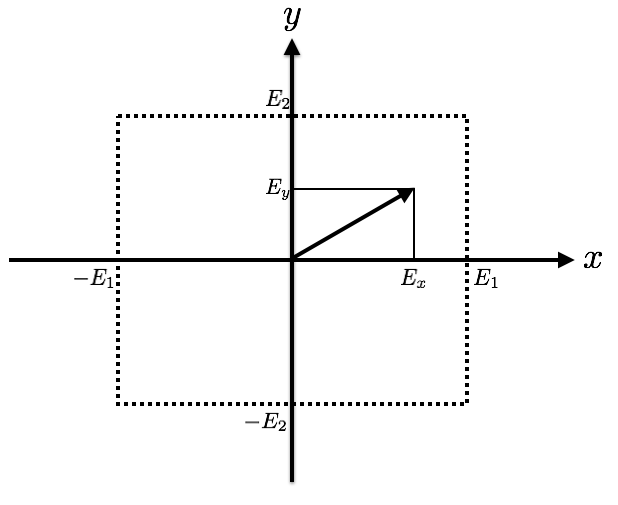
\includegraphics[width=0.65\textwidth]{Pictures/polarizacionxy.png}
\caption{\textit{Polarizaci\'on lineal.}}
\end{figure}


la cual representa la ecuaci\'on de una recta con pendiente $\frac{E_1}{E_2}$. La punta del vector $\textbf{E}_0$ siempre se encuentra
sobre est\'a l\'inea (ver figura) y se dice que este campo est\'a \textit{linealmente polarizado.}
\end{itemize}

\begin{itemize}
 \item Para el caso en que $|\vartheta_2-\vartheta_1|=\pi$, la ecuaci\'on (\ref{ec elipse}) queda como,
\begin{equation*}
\left( \frac{E_x}{E_1} + \frac{E_y}{E_2}\right)^2=0,
\end{equation*}
por lo tanto,
\begin{equation}
\frac{E_x}{E_1} = -\frac{E_y}{E_2},
\end{equation}



la cual representa la ecuaci\'on de una recta con pendiente $-\frac{E_1}{E_2}$. Al tener la misma pendiente pero con signo contrario que
el ejemplo anterior, la polarizaci\'on es lineal pero perpendicular a la anterior,
 \end{itemize}

\begin{figure}[h!]
\centering
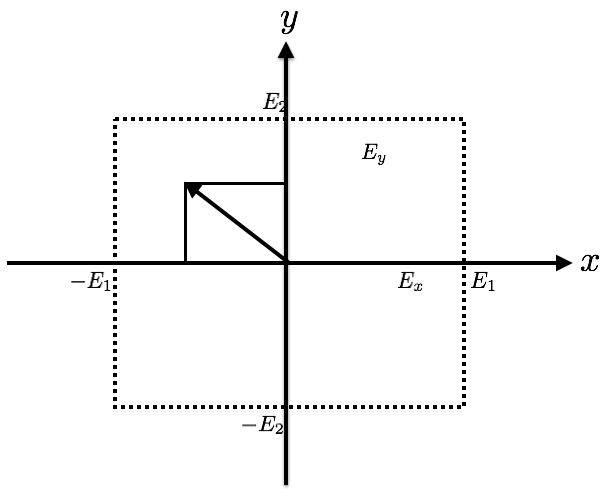
\includegraphics[width=0.65\textwidth]{Pictures/polarizacionnegatica.png}
\caption{Polarizaci\'on lineal con pendiente negativa.}
\end{figure}

\begin{itemize}
 \item Por ultimo cuando $|\vartheta_2-\vartheta_1|=\frac{\pi}{2}$, la ecuaci\'on (\ref{ec elipse}) toma la forma,
\begin{equation*}
\left( \frac{E_x}{E_1}\right)^2 + \left(\frac{E_y}{E_2}\right)^2=1,
\end{equation*}
la cual representa la ecuaci\'on de una elipse con los ejes alineados a los ejes. Este tipo de polarizaci\'on se conoce como
\textit{polarizaci\'on el\'iptica.} \\\\

\begin{figure}[h!]
\centering
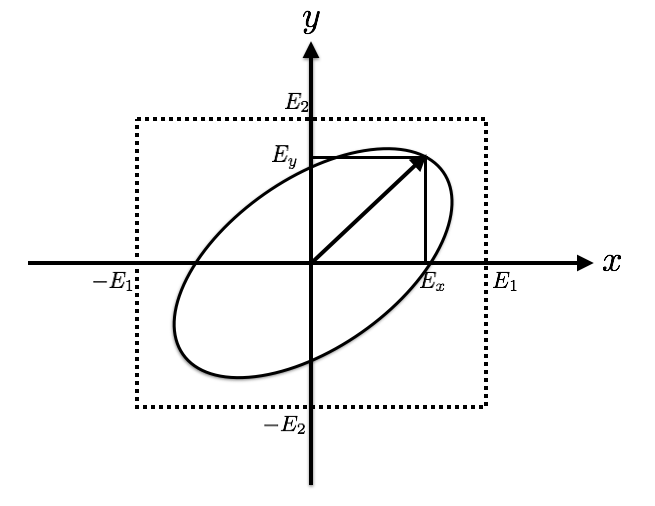
\includegraphics[width=0.65\textwidth]{Pictures/polarizacioneliptica.png}
\caption{Polarizaci\'on eliptica.}
\end{figure}

Un caso especial de este tipo de polarizaci\'on es cuando $E_1=E_2=E_0$, por lo tanto la expresi\'on (\ref{ec elipse}) toma la forma,
\begin{equation}
 E_x^2+E_y^2=E_o^2,
\end{equation}
es la ecuaci\'on de una circunferencia, entonces se dice que el campo el\'ectrico est\'a \textit{polarizado circularmente.}

\begin{figure}[h!]
\centering
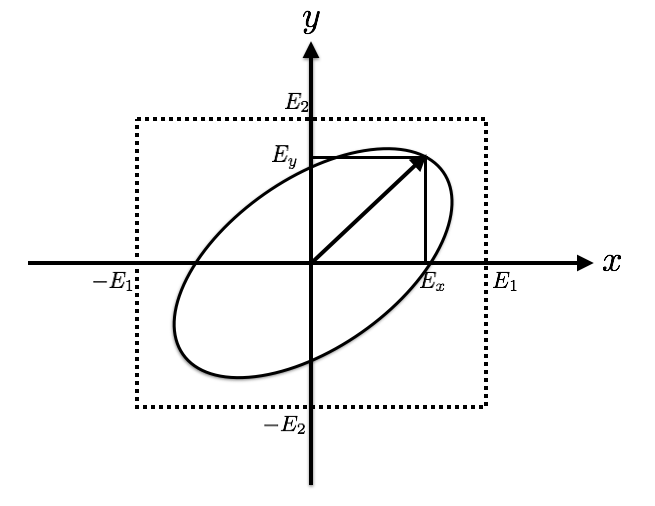
\includegraphics[width=0.65\textwidth]{Pictures/polarizacioneliptica.png}
\caption{\textit{Polarizaci\'on eliptica.}}
\end{figure}
 \end{itemize}

\section{En medios diel\'ectricos: \'Indice de refracci\'on; velocidades de fase y transporte de energ\'ia.}
Hasta ahora, solo se ha analizado los casos cuando los campos el\'ectricos y magn\'eticos se encuentran en el vac\'io, veamos ahora
lo que sucede cuando se mueven por materiales diel\'ectricos.\\
La ecuaci\'on de onda en este caso es:
\begin{equation}
 \nabla^2 \psi-\epsilon\mu\frac{\partial^2 \psi}{\partial t^2}=0,
\end{equation}
del mismo modo, se define una velocidad de propagaci\'on, $\mbox{v}$, definida como $\mbox{v}=\frac{1}{\sqrt{\epsilon\mu}}$.
\subsection{\'Indice de refracci\'on.}
Es com\'un expresar la velocidad de propagaci\'on $v$ como,
\begin{equation}
v=\frac{c}{n},
\end{equation}
de modo que,
\begin{eqnarray*}
\begin{split}
\frac{c}{n}&=\frac{1}{\sqrt{\epsilon \mu}},\\
&=\frac{1}{\sqrt{k_{e}\epsilon_{0} k_m\mu_0}},\\
&=\frac{1}{\sqrt{\epsilon_0\mu_0}\sqrt{K_mK_e}},
\end{split}
\end{eqnarray*}

por la tanto,
\begin{equation}
n=\sqrt{K_mK_e}.
\end{equation}
Donde $n$ se le denomina \textit{indice re refracci\'on}, cuando $n=1$, el medio de propagaci\'on es el vac\'io.
El tratamiento de la propagaci\'on de ondas en medios diel\'ectricos es semejante al ya hecho en el vac\'io, lo \'unico que hay que considerar, es el cambio en la velocidad de fase.\\
\subsection{Velocidad de fase y densidad de energ\'ia}

Analizando de manera similar la expresi\'on (\ref{psi}),
\begin{equation*}
\psi=\psi_0\text{e}^{i(\textbf{k}\cdot\textbf{r}-\omega t)},
\end{equation*}
donde $\psi_0$ tiene la forma,
\begin{equation*}
\psi_0=\psi_{0r}\text{e}^{i\vartheta},
\end{equation*}
donde $\vartheta$ es el \'angulo de fase de la onda plana, entonces,
\begin{equation*}
\psi=\psi_{0r}\text{e}^{i(\textbf{k}\cdot\textbf{r}-\omega t+\vartheta)},
\end{equation*}
tomando la parte real de $\psi$ y analizando su periodicidad tanto en el espacio como en el tiempo, de tal manera que,
\begin{eqnarray*}
\begin{split}
\psi(x,t)=&\psi(x\pm\lambda,t),\\
\psi(x,t)=&\psi(x,t\pm\tau),
\end{split}
\end{eqnarray*}
esto ocurre si, $k=\frac{2\pi}{\lambda}$ y $\omega=\frac{2\pi}{\tau}$, como $\omega=kv$,
\begin{equation*}
\frac{2\pi}{\tau}=\frac{2\pi}{\lambda}v,
\end{equation*}
es decir,
\begin{equation*}
\nu=\frac{v}{\lambda}
\end{equation*}
donde, $\nu$, es la frecuencia, definida como el inverso de $\tau$, por lo tanto obtenemos,
\begin{equation}
v=\lambda\nu
\end{equation}
Ahora bien, el promedio temporal del vector de Poynting esta definido como,
\begin{equation*}
\langle\textbf{S} \rangle=\frac{1}{2}\text{Re  }(\textbf{E}\times \textbf{H}^{*})
\end{equation*}
mientras que la densidad de energ\'ia electromagn\'etica como,
\begin{equation}
\langle u \rangle =\frac{\epsilon}{4}(\textbf{E}\cdot\textbf{E}^{*})+\frac{\mu}{4}(\textbf{H}\cdot\textbf{H}^{*})
\end{equation}


\begin{example}
Obtenga las relaciones de energ\'ia para una onda plana en un medio diel\'ectrico.\\\\
Soluci\'on.\\\\

Sabemos que el prmedio temporal del vector de Poynting es,
\begin{equation*}
\langle \textbf{S} \rangle= \frac{1}{2}\text{Re  }(\textbf{E}\times \textbf{H}^{*}),
\end{equation*}
sustituyendo la expresi\'on (\ref{H_z}) para el campo magn\'etico, donde $Z=\left(\frac{\mu}{\epsilon}\right)^{1/2}$, la impedancia en el medio,
\begin{equation*}
\begin{split}
\langle \textbf{S} \rangle=&\frac{1}{2}\text{Re  }\left[ \textbf{E}\times \left( \frac{\hat{\textbf{n}}\times \textbf{E}^{*}}{Z} \right)\right],\\
=&\frac{1}{2}\left(\frac{\epsilon}{\mu}\right)^{1/2}\text{Re  }\left[  (\textbf{E}\cdot\textbf{E}^{*})\hat{\textbf{n}}-(\hat{\textbf{n}}\cdot\textbf{E})\textbf{E}^{*}  \right],\\
=&\frac{1}{2}\left(\frac{\epsilon}{\mu}\right)^{1/2}\text{Re  }\left[ (\textbf{E}\cdot\textbf{E}^{*})\hat{\textbf{n}} \right],\\
\end{split}
\end{equation*}
puesto que $\hat{\textbf{n}}\cdot\textbf{E}$ es una de las condiciones de frontera, ya que el campo $\textbf{E}$ siempre es perpendicular a la direcci\'on de propagaci\'on $\hat{\textbf{n}}$. Adem\'as como, $\textbf{E}\cdot\textbf{E}^{*}$ es el modulo de $\textbf{E}$ este ya es una cantidad real, por lo tanto,
\begin{equation*}
\langle \textbf{S} \rangle=\frac{1}{2}\left(\frac{\epsilon}{\mu}\right)^{1/2}|\textbf{E}|^2 \hat{\textbf{n}},
\end{equation*}
Ahora,  si vemos a los campos $\textbf{E}$ y $\textbf{H}$ como exponenciales complejas, sabemos que $|\textbf{E}|^2=|E_0|^2$ y $|\textbf{H}|^2=|H_0|^2$, por la tanto,
\begin{equation*}
\langle \textbf{S} \rangle=\frac{1}{2}\left(\frac{\epsilon}{\mu}\right)^{1/2}|E_0|^2 \hat{\textbf{n}},
\end{equation*}
se puede hacer de forma an\'aloga para $\textbf{H}$, de modo que,
\begin{equation*}
\langle \textbf{S} \rangle=\frac{1}{2}\left(\frac{\epsilon}{\mu}\right)^{1/2}|H_0|^2 \hat{\textbf{n}},
\end{equation*}
 por la tanto, la densidad del flujo de energ\'ia tiene la direcci\'on de propagaci\'on y es proporcional al cuadrado de la amplitud de $\textbf{E}$ o $\textbf{H}$. Ahora si calculamos la densidad de energ\'ia promedio obtenemos,
\begin{equation*}
\begin{split}
\langle u \rangle =&\frac{\epsilon}{4}(\textbf{E}\cdot\textbf{E}^{*})+\frac{\mu}{4}(\textbf{H}\cdot\textbf{H}^{*}),\\
=&\frac{\epsilon}{4}|E_0|^2+\frac{\mu}{4}\frac{\epsilon}{4}|H_0|^2,\\
=&\frac{\epsilon}{2}|E_0|^2=\frac{\epsilon}{2}|H_0|^2,
\end{split}
\end{equation*}
si sustituimos este resultado en la expresi\'on obtenida para el vector de Poynting,
\begin{equation*}
\begin{split}
\langle \textbf{S} \rangle=&\frac{1}{2}\left(\frac{\epsilon}{\mu}\right)^{1/2}|H_0|^2 \hat{\textbf{n}},\\
=&\frac{1}{2}\left(\frac{\epsilon}{\mu}\right)^{1/2}\frac{2\langle u \rangle}{\mu} \hat{\textbf{n}},\\
=&\frac{\langle u \rangle}{\sqrt{\epsilon\mu}}\hat{\textbf{n}}.
\end{split}
\end{equation*}
\begin{equation}
\langle \textbf{S} \rangle=\langle u \rangle \textbf{v}.
\end{equation}
As\'i la densidad del flujo promedio de la energ\'ia es igual al valor promedio de la densidad de energ\'ia multiplicada por la velocidad de propagaci\'on de la onda, lo que recuerda un poco con la densidad de corriente $\textbf{J}=\rho \textbf{v}$.

\end{example}

\section{Ley de refracci\'on y de reflexi\'on, ecuaciones de Fresnel; efectos de polarizaci\'on; reflexi\'on total interna y ondas evanescentes.}
Hasta ahora, solo hemos considerado regiones en donde no tenemos densidades de carga y densidades de corriente, o los campos est\'an muy alejados de las fuentes. Consideremos como estas fuentes afectan a los campos vistos como una fuente de ondas planas.

 \subsection{Ley de refracci\'on Y reflexi\'on}
 Se consideran dos medios separados por un plano infinito, sin cargas y corrientes libres, las componentes de los campos $\textbf{D}$ y $\textbf{H}$ se pueden calcular como ya se habia hecho antes en los c\'apitulos pasados, adem\'as se tienen las condiciones que caracterizan cada medio, ($\epsilon,\mu,\sigma$),

Suponemos que estamos trabajando con medios no conductores, es decir, $\sigma=0$, ademas se supone que para que las condiciones de frontera se cumplan, si tiene que tener tres odas planas; la incidente, la reflejada en el medio 1 y la transmitida en el medio 2. Por medio de la ecuaci\'on (\ref{}),
\begin{equation}
\begin{split}
\textbf{E}_i=&\textbf{E}_{0i}\text{e}^{i(\textbf{k}_i\cdot\textbf{r}-\omega_i t) },\\
\textbf{E}_r=&\textbf{E}_{0r}\text{e}^{i(\textbf{k}_r\cdot\textbf{r}-\omega_r t) },\\
\textbf{E}_t=&\textbf{E}_{0t}\text{e}^{i(\textbf{k}_t\cdot\textbf{r}-\omega_t t) },
\end{split}
\end{equation}
de manera que,
\begin{equation}
\begin{split}
k_i^2=\left(  \frac{\omega_i}{v_1} \right)^2=\left(  \frac{n_1\omega_i}{c} \right)^2,\\
k_r^2=\left(  \frac{\omega_r}{v_1} \right)^2=\left(  \frac{n_1\omega_r}{c} \right)^2,\\
k_t^2=\left(  \frac{\omega_t}{v_2} \right)^2=\left(  \frac{n_2\omega_r}{c} \right)^2,\\
\end{split}
\end{equation}
Por lo tanto, el campo el\'ectrico en cualquier punto de la regi\'on 1 es,  $\textbf{E}_1=\textbf{E}_i+\textbf{E}_r$, mientras que el campo en la regi\'on 2 es $\textbf{E}_2=\textbf{E}_t$, de modo que las componentes tangenciales en la interfase tienen que ser iguales, obteniendo,
\begin{equation}
\textbf{E}_i=\textbf{E}_{0i}\text{e}^{i(\textbf{k}_i\cdot\textbf{r}-\omega_i t) }+\textbf{E}_{0r}\text{e}^{i(\textbf{k}_r\cdot\textbf{r}-\omega_r t) }=\textbf{E}_{0t}\text{e}^{i(\textbf{k}_t\cdot\textbf{r}-\omega_t t) }
\end{equation}
para que esta ecuaci\'on se cumpla, las exponentes tienen que ser iguales, de manera que, $\omega_i=\omega_r=\omega_t=\omega$, de manera que las expresiones de la ecuaci\'on () se transforman en,
\begin{equation}
\begin{split}
k_i^2=\left(  \frac{n_1\omega}{c} \right)^2=k_1^2,\\
k_r^2=\left(  \frac{n_1\omega}{c} \right)^2=k_1^2\\      \label{Cuadra}
k_t^2=\left(  \frac{n_2\omega}{c} \right)^2=k_2^2\\
\end{split}
\end{equation}

\begin{figure}[hbtp]
\centering
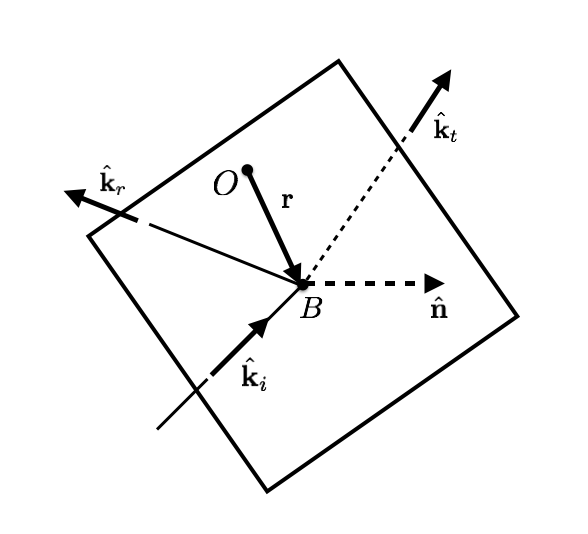
\includegraphics[scale=0.4]{Pictures/Relsuperficie.png}
\caption{Relaciones en una superficie plana entre dos medios}
\end{figure}


De la misma manera pasa con $\textbf{k}_i \cdot \textbf{r}=\textbf{k}_r \cdot \textbf{r}=\textbf{k}_t \cdot \textbf{r}$, de modo que obtenemos,
\begin{equation}
(\textbf{k}_i-\textbf{k}_r)\cdot\textbf{r}=0,  \label{LeyReflexion}
\end{equation}
\begin{equation}
(\textbf{k}_i-\textbf{k}_t)\cdot\textbf{r}=0,  \label{LeyRefraccion}
\end{equation}
esto es, que las diferencias entre los vectores de propagaci\'on son perpendiculares con el vector $\textbf{r}$, el cual se encuentra sobre el plano de incidencia. La ec (\ref{LeyReflexion}) nos brinda una realaci\'on entre la onda incidente y la reflejada, por lo cual se le conoce con el nombre de \textit{ley de reflexi\'on.} Mientas que la expresi\'on (\ref{LeyRefraccion}) nos proporciona informaci\'on de los vectores de propagaci\'on incidente y trasmitido, por lo que se le conoce como \textit{ley de refracci\'on.}\\
El plano formado por los vectores $\textbf{k}_i$ y $\hat{\textbf{n}}$ recibe el nombre de plano de incidencia. De modo que el \'angulo formado entre estos dos vectores se le conoce como \textit{\'angulo de incidencia.} \\
Podemos descomponer el vector $\textbf{k}_i$ en sus componentes normal y paralela a la superficie de la interfase, si se introdce un vector $\hat{\mathbf{\tau}}$ unitario de modo que este se encuentre sobre el plano de incidencia, por lo tanto,
\begin{equation}
\textbf{k}_i=k_{in}\hat{\textbf{n}}+k_{i\tau}\hat{\mathbf{\tau}},
\end{equation}
An\'alogamente se puede descomponer cualquier otro vector si se define un nuevo vector $\hat{\textbf{n}}\times\hat{\mathbf{\tau}}$ unitario que se encuentra tambi\'en obre la superficie del plano de incidencia, ver figura, de modo que es posible expresar los vectores $\textbf{k}_r$, $\textbf{k}_t$ y $\textbf{r}$, obteniendo,

\begin{figure}[hbtp]
\centering
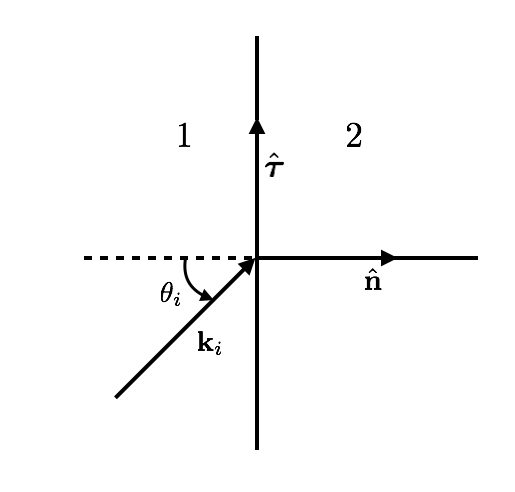
\includegraphics[scale=0.4]{Pictures/Plano_incidencia.png}
\caption{Plano de incidencia.}
\end{figure}


\begin{equation}
\textbf{k}_r=k_{rn}\hat{\textbf{n}}+k_{r\tau}\hat{\mathbf{\tau}}+k_{rc}(\hat{\textbf{n}}\times\hat{\mathbf{\tau}}),  \label{kr}
\end{equation}
\begin{equation}
\textbf{k}_t=k_{tn}\hat{\textbf{n}}+k_{t\tau}\hat{\mathbf{\tau}}+k_{tc}(\hat{\textbf{n}}\times\hat{\mathbf{\tau}}),  \label{kt}
\end{equation}
\begin{equation}
\textbf{r}=r_{\tau}\hat{\mathbf{\tau}}+r_c(\hat{\textbf{n}}\times\hat{\mathbf{\tau}}),
\end{equation}
sustituyendo en las ecuaciones (\ref{LeyReflexion}), obtenemos,
\begin{equation*}
(\textbf{k}_i-\textbf{k}_r)\cdot\textbf{r}=[k_{in}\hat{\textbf{n}}+k_{i\tau}\hat{\mathbf{\tau}}-(k_{rn}\hat{\textbf{n}}+k_{r\tau}\hat{\mathbf{\tau}}+k_{rc}(\hat{\textbf{n}}\times\hat{\mathbf{\tau}}))]\cdot[r_{\tau}\hat{\mathbf{\tau}}+r_c(\hat{\textbf{n}}\times\hat{\mathbf{\tau}})],
\end{equation*}
agrupando t\'erminos,
\begin{equation*}
[(k_{in}-k_{rn})\hat{\textbf{n}}+(k_{i\tau}-k_{r\tau})\hat{\mathbf{\tau}}-k_{rc}(\hat{\textbf{n}}\times\hat{\mathbf{\tau}})]\cdot[r_{\tau}\hat{\mathbf{\tau}}+r_c(\hat{\textbf{n}}\times\hat{\mathbf{\tau}})]=0,
\end{equation*}
ahora si sustituimos en (\ref{LeyRefraccion}) de forma similar encontramos que,
 \begin{equation}
 \begin{split}
(k_{in}-k_{rn})r_{\tau}-k_{rc}r_{c}=&0,\\
(k_{i\tau}-k_{t\tau})r_{\tau}-k_{tc}r_{c}=&0. \label{Leyes2}
\end{split}
 \end{equation}

 \begin{obs}
Dado que $\textbf{r}$ es un vector cualquiera sobre el plano de incidencia, las expresiones (\ref{Leyes2}) deber ser ciertas para el caso $r_{\tau}=0$ con $r_c\neq0$, encontrando que,
\begin{equation}
k_{rc}=k_{tc}=0,
\end{equation}
es decir, que $\textbf{k}_r$ y $\textbf{k}_{\tau}$ se encuentran sobre el plano de incidencia y no tienen componentes perpendiculares al plano de la figura (\ref{1ab}),m por otro lado, ya que $r_c\neq0$, de la ec. (\ref{Leyes2}) obtenemos,
 \begin{equation}
 \begin{split}
k_{in}-k_{rn}=&0,\\
k_{i\tau}-k_{t\tau}=&0,
\end{split}
 \end{equation}
estas dos relaciones se suelen considerar como una segunda version de las leyes de reflexi\'on y reflacci\'on.
\end{obs}
Estudiando ahora las componentes normales de los vectores de propagaci\'on encontramos que $k_{rc}=0$, por lo tanto, las ecuaciones (\ref{kr}) y (\ref{kt}) se pueden reescribir como,

\begin{equation*}
\begin{split}
\textbf{k}_r=&k_{rn}\hat{\textbf{n}}+k_{r\tau}\hat{\mathbf{\tau}},\\
\textbf{k}_t=&k_{tn}\hat{\textbf{n}}+k_{t\tau}\hat{\mathbf{\tau}},
\end{split}
\end{equation*}
recordando de las ecuaciones (\ref{Cuadra}) y calculando los m\'odulos al cuadrado de $\textbf{k}_r$ y $\textbf{k}_t$, encontramos que $k_i^2=k_r^2=k_{in}^2+k_{i\tau}^2=k_{rn}^2+k_{r\tau}^2$,
\begin{equation*}
\begin{split}
k_{in}^2&=k_r^2-k_{i\tau}^2,\\
&=k_r^2-k_{i\tau}^2,\\
&=k_i^2-k_{i\tau}^2,\\
\end{split}
\end{equation*}

\begin{equation*}
\begin{split}
k_{rn}^2&=k_r^2-k_{i\tau}^2,\\
&=k_r^2-k_{i\tau}^2,\\
&=k_i^2-k_{i\tau}^2,\\
\end{split}
\end{equation*}
por lo tanto, $k_{in}^2=k_{rn}^2$, al sacar ra\'ices tenemos, $k_{rn}=\pm k_{in}$, dado que la onda reflejada viaja en sentido contrario a la onda incidente, se toma el signo negativo, por lo cual se encuentra que,
\begin{equation}
k_{rn}=-K_{in}. \label{Refle}
\end{equation}
Podemos hacer algo similar para el vector propagaci\'on de la onda transmitida,

\begin{equation}
\begin{split} \label{Refla}
k_{tn}^2=&k_t^{2}-t_{t\tau}^2,\\
=&k_{2}^2-t_{t\tau}^2,
\end{split}
\end{equation}
las ecuaciones (\ref{Refle}) y (\ref{Refla}), forman uyna tercera versi\'on de las leyes de reflexi\'on y reflacci\'on.

\begin{figure}[hbtp]
\centering
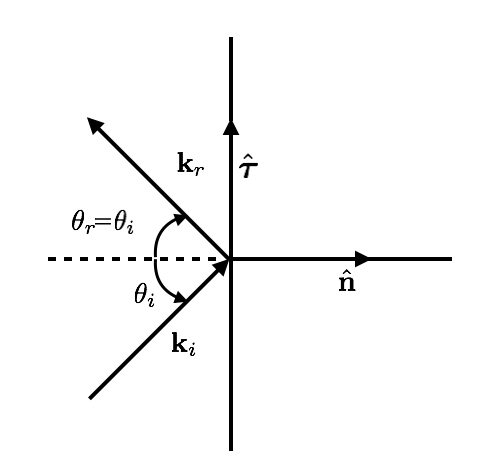
\includegraphics[scale=0.4]{Pictures/Angulo_i_r.png}
\caption{Vectores de propagaci\'on incidente y reflejado}
\end{figure}

Dada la figura (tal) podemos observar que,
\begin{equation*}
\begin{split}
k_{in}=&k_1 \cos\theta_i,\\
k_{i\tau}=&k_1  \sen \theta_i,
\end{split}
\end{equation*}
 por lo tanto
\begin{equation*}
\begin{split}
k_{rn}=&-k_1 \cos\theta_i,\\
k_{r\tau}=&k_1  \sen \theta_i,
\end{split}
\end{equation*}
 y dado que $ \textbf{k}_r$ tiene la misma magnitud que $\textbf{ k}_i$, podemos definir una \'angulo de reflexi\'on, $\theta_r$, tal que,
\begin{equation*}
\begin{split}
k_{rn}=&-k_1 \cos\theta_r,\\
k_{r\tau}=&k_1  \sen \theta_r,
\end{split}
\end{equation*}
 por comparaci\'on podemos ver que,
 \begin{equation}
 \theta_i=\theta_r,
 \end{equation}
de modo que el \'angulo de incidencia resulta ser igual al \'angulo de reflexi\'on, es as\'i que una de las muy conocidas leyes de \'optica resulta ser una consecuencia de las ecuaciones de Maxwell.  Para la onda transmitida, se sabe que, $k_{t\tau}=k_{i\tau}$, obteniendo $k_{t\tau}=k_1 \sen \theta_i$.
Recordando la ec. (\ref{Refla}),
\begin{equation*}
\begin{split}
k_{tn}^2=&k_{2}^2-t_{t\tau}^2,\\
=&k_2^2-k_1^2 \sen ^2 \theta_i,\\
=& k_2^2 \left[ 1-\left( \frac{k_1}{k_2}  \right)^2 \sen ^2 \theta_i \right],\\
=& k_2^2 \left[ 1-\left( \frac{n_1}{n_2}  \right)^2 \sen ^2 \theta_i \right]
\end{split}
\end{equation*}
en ocasiones resulta \'util introducir un \'angulo de reflacci\'on, $\theta_t$, de modo que,
\begin{equation*}
\begin{split}
k_{t\tau}=&k_2 \sen \theta_{t},\\
k_{tn}=&k_2 \cos \theta_{t}.\\
\end{split}
\end{equation*}
 Recordando la relaci\'on $k_{i\tau}=k_{t\tau}$, con los resultados obtenidos,
 \begin{equation*}
 k_1 \sen \theta_i=k_2 \sen \theta_t,
 \end{equation*}
si sustituimos los valores de $k_1$ y $k_2$,
 \begin{equation*}
\frac{\omega n_1}{c} \sen \theta_i=\frac{\omega n_2 }{c} \sen \theta_t,
 \end{equation*}
resultando,
\begin{equation}
n_1\sen \theta_i=n_2\sen \theta_t,
\end{equation}
la conocida \textit{ley de reflacci\'on de Snel.}

\subsection{Ecuaciones de Fresnell}
Si suponemos de nuevo dos medios separados por una interfase y los campos $\textbf{E}$ y $\textbf{H}$como se indica en la figura,\\\\
Dado que los campos el\'ectricos son paralelos entre si, sabemos que sus componentes tangenciales son iguales,
\begin{equation*}
 \textbf{E}_{1_{tangencial}}=\textbf{E}_{2_{tangencial}},
 \end{equation*}
esto es,
\begin{equation}
\textbf{E}_i+\textbf{E}_r=\textbf{E}_t, \label{E_frontera}
\end{equation}


adem\'as las campos magn\'eticos $\textbf{H}$ est\'an sobre el plano de incidencia con $\hat{\tau}$, un vector tangente unitario a est\'a, entonces so condici\'on de frontera es,
\begin{equation*}
 \textbf{H}_{1_{tangencial}}=\textbf{H}_{2_{tangencial}},
 \end{equation*}
o bien,
\begin{equation}
(\textbf{H}_i+\textbf{H}_r)\cdot \hat{\tau}=\textbf{H}_t\cdot \hat{\tau}, \label{H_frontera}
\end{equation}
est\'a ultima expresi\'on puede ser reescrita con ayuda de, $\textbf{H}=\frac{\hat{\textbf{k}}\times\textbf{E}}{Z}$ y $\hat{\tau}=\frac{\textbf{E}_i\times\hat{\textbf{n}}}{E_i}$, por lo tanto,

\begin{equation*}
\begin{split}
\textbf{H}\cdot \hat{\tau}=&\left(\frac{\hat{\textbf{k}}\times\textbf{E}}{Z}\right)\cdot\left( \frac{\textbf{E}_i\times\hat{\textbf{n}}}{E_i} \right).\\
=&\frac{1}{ZE_i}(\hat{\textbf{k}}\times\textbf{E})\cdot(\textbf{E}_i\times\hat{\textbf{n}}),\\
=&\frac{1}{ZE_i} \left[ (\hat{\textbf{k}}\cdot\textbf{E}_i)(\textbf{E}\cdot\hat{\textbf{n}})-(\hat{\textbf{k}}\cdot\hat{\textbf{n}})(\textbf{E}\cdot\textbf{E}_i) \right],
\end{split}
\end{equation*}
 recordando de las condiciones de frontera $\textbf{E}_i\cdot\textbf{k}=0$ y $\textbf{E}$ es paralelo a $\textbf{E}_i$, la expresi\'on anterior se reduce a,
 \begin{equation*}
\textbf{H}\cdot \hat{\tau}=-\frac{E}{Z}(\hat{\textbf{k}}\cdot\hat{\textbf{n}}),
 \end{equation*}
entonces podemos reescribir la ec. (\ref{H_frontera}) como,
\begin{equation} \label{desarrollo}
\frac{1}{Z_1}\left[E_1(\hat{\textbf{k}_i}\cdot\hat{\textbf{n}})+E_r(\hat{\textbf{k}_r}\cdot\hat{\textbf{n}})\right]=\frac{1}{Z_2}E_t(\hat{\textbf{k}_t}\cdot\hat{\textbf{n}})
\end{equation}
si multiplicamos todo por $\frac{1}{E_1}$ y sustituimos la ec. (\ref{E_frontera}),

\begin{equation*}
\begin{split}
\frac{1}{Z_1}\left[\hat{\textbf{k}_i}\cdot\hat{\textbf{n}}+\frac{E_r}{E_i}(\hat{\textbf{k}_r}\cdot\hat{\textbf{n}})\right]=&\frac{1}{Z_2}\frac{E_i+E_r}{E_i}(\hat{\textbf{k}_t}\cdot\hat{\textbf{n}}),\\
\frac{1}{Z_1}\left[\hat{\textbf{k}_i}\cdot\hat{\textbf{n}}+\frac{E_r}{E_i}(\hat{\textbf{k}_r}\cdot\hat{\textbf{n}})\right]=&\frac{1}{Z_2}\left(1+\frac{E_r}{E_i}\right)(\hat{\textbf{k}_t}\cdot\hat{\textbf{n}}),\\
\end{split}
\end{equation*}
desarrollando un poco los t\'erminos,
\begin{equation*}
\begin{split}
Z_2\left[\hat{\textbf{k}_i}\cdot\hat{\textbf{n}}+\frac{E_r}{E_i}(\hat{\textbf{k}_r}\cdot\hat{\textbf{n}})\right]-Z_1\left(1+\frac{E_r}{E_i}\right)(\hat{\textbf{k}_t}\cdot\hat{\textbf{n}})=&0,\\
Z_2(\hat{\textbf{k}_i}\cdot\hat{\textbf{n}})+Z_2\frac{E_r}{E_i}(\hat{\textbf{k}_r}\cdot\hat{\textbf{n}})-Z_1(\hat{\textbf{k}_t}\cdot\hat{\textbf{n}})-Z_1\frac{E_r}{E_i}(\hat{\textbf{k}_t}\cdot\hat{\textbf{n}})=&0,\\
\end{split}
\end{equation*}
despejando $\frac{E_r}{E_i}$, obtenemos,
\begin{equation*}
\begin{split}
\frac{E_r}{E_i}&\left[ Z_2(\hat{\textbf{k}_r}\cdot\hat{\textbf{n}})-Z_1(\hat{\textbf{k}_t}\cdot\hat{\textbf{n}})\right]=Z_1(\hat{\textbf{k}_t}\cdot\hat{\textbf{n}})-Z_2(\hat{\textbf{k}_i}\cdot\hat{\textbf{n}}),\\
\frac{E_r}{E_i}&=\frac{Z_1(\hat{\textbf{k}_t}\cdot\hat{\textbf{n}})-Z_2(\hat{\textbf{k}_i}\cdot\hat{\textbf{n}})}{Z_2(\hat{\textbf{k}_r}\cdot\hat{\textbf{n}})-Z_1(\hat{\textbf{k}_t}\cdot\hat{\textbf{n}})},
\end{split}
\end{equation*}
de modo que, si se hace uso de, $\hat{\textbf{k}}_r\cdot\hat{\textbf{n}}=-\hat{\textbf{k}}_i\cdot\hat{\textbf{n}}$ encontramos,

\begin{equation}  \label{E_r}
\left(\frac{E_r}{E_i}\right)_{\perp}=\frac{Z_2(\hat{\textbf{k}_i}\cdot\hat{\textbf{n}})-Z_1(\hat{\textbf{k}_t}\cdot\hat{\textbf{n}})}{Z_2(\hat{\textbf{k}_i}\cdot\hat{\textbf{n}})+Z_1(\hat{\textbf{k}_t}\cdot\hat{\textbf{n}})}.
\end{equation}
De mismo modo podemos partir de la ec. (\ref{desarrollo}) y calcular $\frac{E_t}{E_i}$,
\begin{equation*}
\begin{split}
Z_2\left[ E_i (\hat{\textbf{k}}_i\cdot\hat{\textbf{n}})+(E_t-E_i)((\hat{\textbf{k}}_r\cdot\hat{\textbf{n}})) \right]=&Z_1E_t(\hat{\textbf{k}}_t\cdot\hat{\textbf{n}}),\\
\frac{E_t}{E_i}\left[ Z_1(\hat{\textbf{k}}_t\cdot\hat{\textbf{n}})+Z_2(\hat{\textbf{k}}_i\cdot\hat{\textbf{n}}) \right]=&Z_2(\hat{\textbf{k}}_i\cdot\hat{\textbf{n}})-Z_2(\hat{\textbf{k}}_r\cdot\hat{\textbf{n}}),
\end{split}
\end{equation*}
por lo tanto,
\begin{equation}   \label{E_t}
\left(\frac{E_t}{E_i}\right)_{\perp}=\frac{2Z_2(\hat{\textbf{k}}_i\cdot\hat{\textbf{n}})}{Z_1(\hat{\textbf{k}}_t\cdot\hat{\textbf{n}})+Z_2(\hat{\textbf{k}}_i\cdot\hat{\textbf{n}})}.
\end{equation}
Dado que $\hat{\textbf{k}}_i\cdot\hat{\textbf{n}}=\cos \theta_i$ y $\hat{\textbf{k}}_t\cdot\hat{\textbf{n}}=\cos \theta_t$, si sustituimos en las ecs. (\ref{E_r}) y (\ref{E_t}) tenemos,

\begin{equation}
\begin{split}  \label{fresn}
\left(\frac{E_r}{E_i}\right)_{\perp}=&\frac{Z_2\cos \theta_i-Z_1\cos \theta_t}{Z_2\cos \theta_i+Z_1\cos \theta_t},\\
\left(\frac{E_t}{E_i}\right)_{\perp}=&\frac{2Z_2\cos \theta_i}{Z_1\cos \theta_t+Z_2\cos \theta_i},
\end{split}
\end{equation}

recordando que $Z=\left( \frac{\mu}{\epsilon} \right)^{1/2}$, entonces podemos escribir, $\frac{Z_1}{Z_2}$,

\begin{equation*}
\frac{Z_1}{Z_2}=\frac{\left( \frac{\mu_1}{\epsilon_1} \right)^{1/2}}{\left( \frac{\mu_2}{\epsilon_2} \right)^{1/2}}=\left(\frac{\mu_1\epsilon_2}{\mu_2\epsilon_1}\right)^{1/2}=\left(\frac{\mu_1\mu_2}{\mu_1\mu_2}\frac{\mu_1\epsilon_2}{\mu_2\epsilon_1}\right)^{1/2}=\left(\frac{\mu_1^2\mu_2\epsilon_2}{\mu_2^2\mu_1\epsilon_1}\right)^{1/2}=\frac{\mu_1 n_2}{\mu_2 n_1},
\end{equation*}
ahora si recordamos la ley de Snell $n_1\cos \theta_i=n_2\cos\theta_t$, entonces, $\frac{n_2}{n_1}=\frac{\sen\theta_i}{\sen\theta_t}$. Por lo tanto,
\begin{equation}  \label{Zrelacion}
\frac{Z_1}{Z_2}=\frac{\mu_1}{\mu_2}\frac{\sen\theta_i}{\sen\theta_t}
\end{equation}
ahora, si a la primera de las ecs (\ref{fresn}) factorizamos tanto en el numerado como en el denominador la cantidad de $Z_2\cos\theta_i$,
\begin{equation*}
\left(\frac{E_r}{E_i}\right)_{\perp}=\frac{1- \frac{Z_1\cos\theta_t}{Z_2\cos\theta_i} }{1+ \frac{Z_1\cos\theta_t}{Z_2\cos\theta_i} },\\
\end{equation*}
si sustituimos la ec. (\ref{Zrelacion}) y un poco de \'algebra obtenemos,
\begin{equation} \label{Fres}
\left(\frac{E_r}{E_i}\right)_{\perp}=\frac{\mu_2\tan \theta_t-\mu_1\tan\theta_i}{\mu_2\tan \theta_t+\mu_1\tan\theta_i}
\end{equation}
de manera similar podemos operar y encontrar una expresi\'on para la segunda ec. de (\ref{fresn}),
\begin{equation}  \label{Fresn}
\left(\frac{E_t}{E_i}\right)_{\perp}=\frac{2\mu_2\tan \theta_t}{\mu_2\tan \theta_t+\mu_1\tan\theta_i}
\end{equation}


A las expresiones (\ref{Fres}) y (\ref{Fresn}) se les conoce como \textit{ecuaciones de Fresnell}, las cuales tambi\'en son obetenidad a partir de las ecuaciones de Maxwell al satisfacer algunas condiciones de frontera.\\

Ahora si suponemos que todos los campos magn\'eticos \textbf{H} apuntan hacia dentro de la pagina, comose muestra en la figura (\ref{grafica}),\\
Sabemos que,
\begin{equation*}
\begin{split}
&\textbf{H}=\frac{1}{Z} \hat{\textbf{k}}\times \textbf{E},\\
&\hat{\textbf{k}}\cdot\textbf{E}=0,
\end{split}
\end{equation*}
\begin{figure}[hbtp]
 \centering
 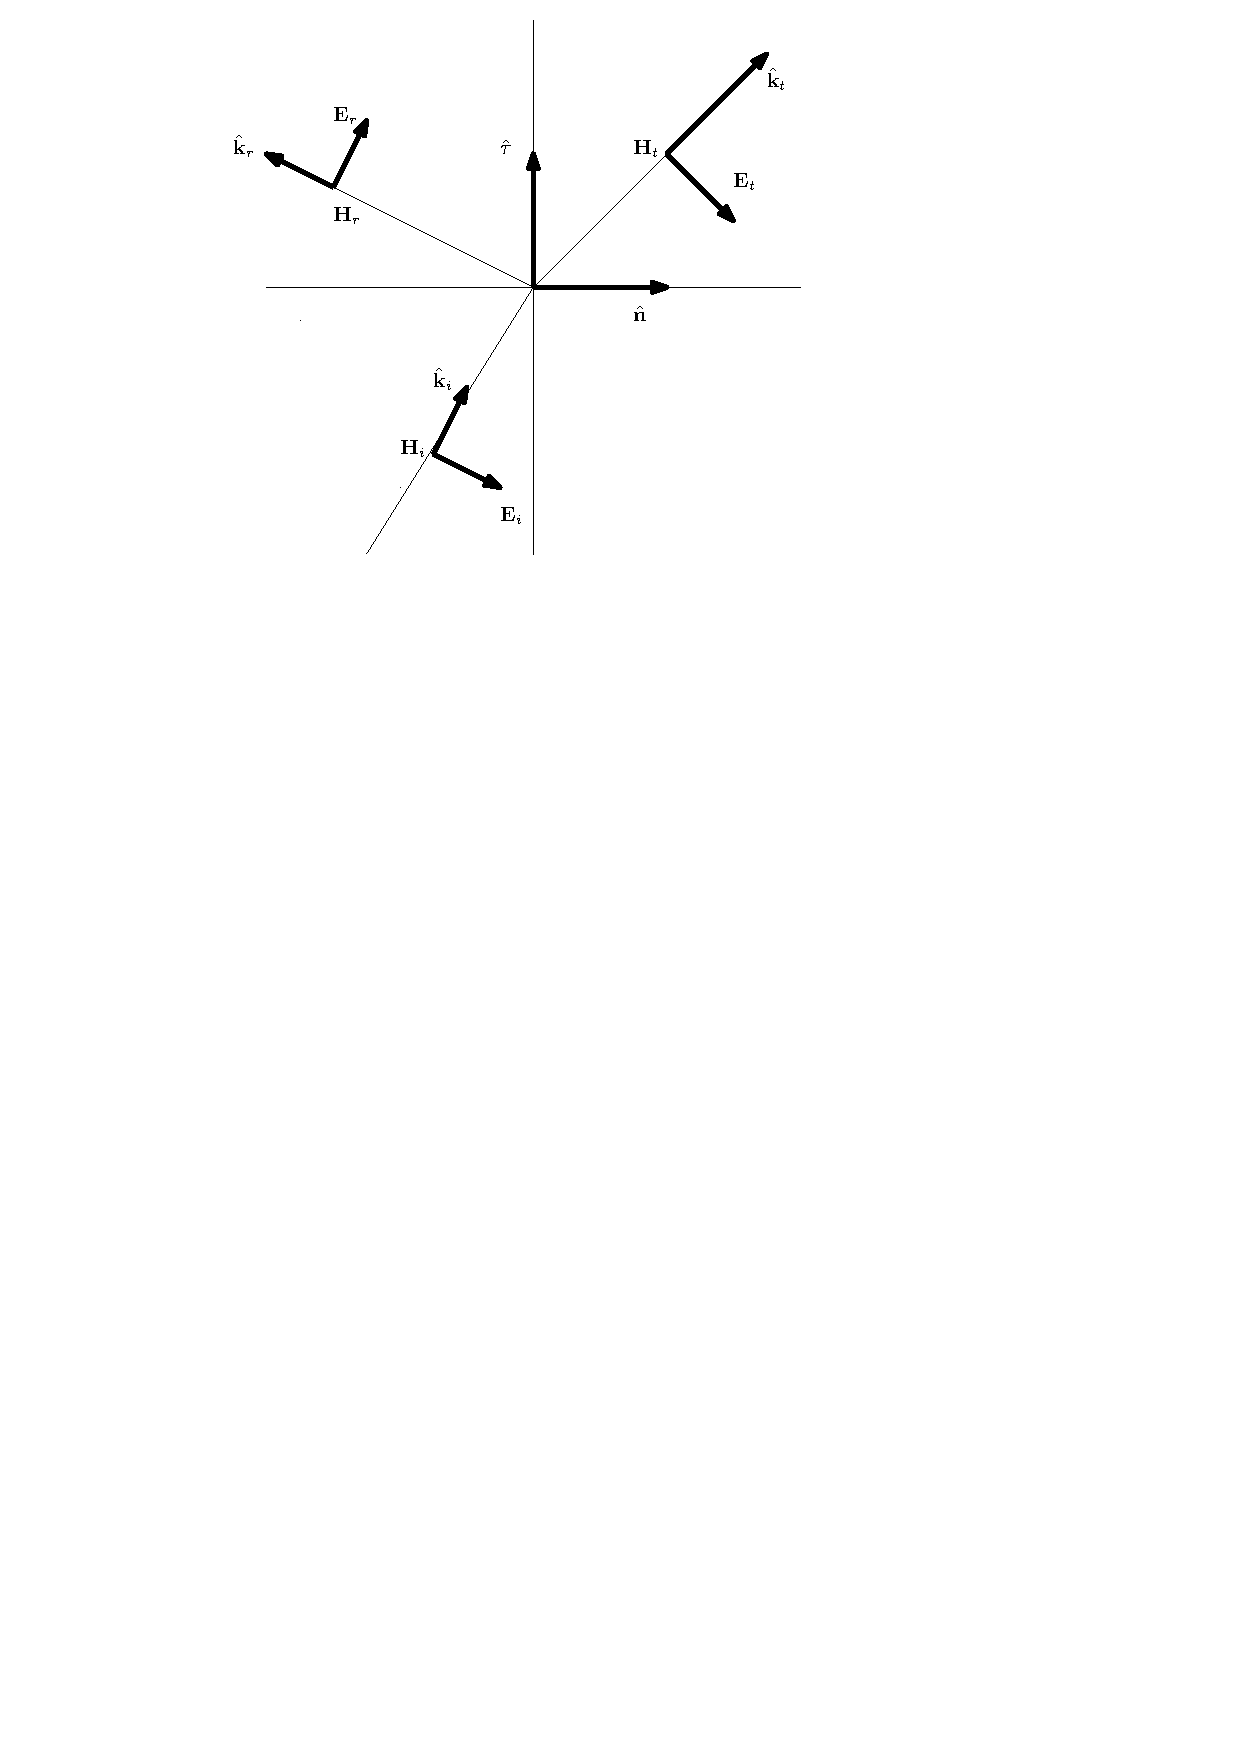
\includegraphics[scale=0.6]{Pictures/fresnell.pdf}
 \caption{$\textbf{E}_{i}$ es paralelo al plano de incidencia}
\label{grafica}
 \end{figure}


\begin{obs}
\begin{equation}
\begin{split}
\textbf{H}\times\hat{\textbf{k}}=&\frac{1}{Z} (\hat{\textbf{k}}\times \textbf{E})\times \hat{\textbf{k}},\\
=&\frac{1}{Z}[\textbf{E}(\hat{\textbf{k}}\cdot\hat{\textbf{k}})-\hat{\textbf{k}}(\hat{\textbf{k}}\cdot\textbf{E})]
\end{split}
\end{equation}
por lo tanto, $\textbf{E}=Z\textbf{H}\times\hat{\textbf{k}}$.
\end{obs}
 Adem\'as podemos ver que $\hat{\tau}=\frac{\hat{\textbf{n}}\times\textbf{H}_i}{H_i}$
\section{En medios conductores: atenuaci\'on y profundidad de la piel; efectos de disipaci\'on.}

 Hasta ahora solo se ha estudiado la ecuaci\'on de ondas cuando $\sigma=0$, ahora supongamos el caso contrario,
 \begin{equation*}
 \nabla^2 \psi(\textbf{r},t)-\mu\sigma\frac{\partial \psi}{\partial t}(\textbf{r},t)-\mu\epsilon \frac{\partial^{2} \psi}{\partial t^{2}}(\textbf{r},t)=0
 \end{equation*}
 Sea $\psi(\textbf{r},t)=\psi_0\text{e}^{i(\textbf{k}\cdot\textbf{r}-\omega t)}$, sustituyendo obtenemos,
 \begin{equation*}
 \psi_0\text{e}^{i(\textbf{k}\cdot\textbf{r}- \omega t)}\left[(i|\textbf{k}|^2)+i\mu\sigma\omega+\mu\epsilon\omega^2\right]=0
 \end{equation*}
obteniendo,
 \begin{equation}  \label{dispersion}
 k^2=\mu\epsilon\omega^2+i\mu\sigma\omega
  \end{equation}
 donde a $k^2$ se le conoce como \textit{relaci\'on de dispersi\'on}, como $k$ es una cantidad compleja, se tiene que,
 \begin{equation*}
 k=\alpha+i\beta
 \end{equation*}
igualando t\'erminos,
 \begin{equation*}
 \alpha^2-\beta^2+2i\alpha\beta=\mu\epsilon\omega^2+i\mu\sigma\omega
 \end{equation*}
 como las partes reales tienen que ser iguales a las partes imaginarias, entonces obtenemos las ecuaciones,
 \begin{equation} \label{1ab}
 \alpha^2-\beta^2=\mu\epsilon\omega^2,
 \end{equation}
 \begin{equation} \label{2ab}
 2\alpha\beta=\mu\sigma\omega,
 \end{equation}
Resolviendo este sistema de ecuaciones,
despejando $\alpha^2$ de (\ref{1ab}),
 \begin{equation*}
 \alpha^2=\mu\epsilon\omega^2+\beta^2
 \end{equation*}
despejando $\beta$ de (\ref{2ab}) y sustituyendo en la anterior,
 \begin{equation*}
 \alpha^2=\mu\epsilon\omega^2+\left( \frac{\omega\sigma\mu}{2 \alpha}\right)^2
 \end{equation*}
ordenando un poco los t\'erminos,
\begin{equation*}
 \alpha^{4}-\mu \epsilon \omega ^{2} \alpha^{2}-\left( \frac{\omega \sigma \mu}{2 \alpha} \right)^2=0
\end{equation*}
sea $m^2=\alpha^4$, obtenemos
\begin{equation*}
m^{2}-\mu\epsilon\omega^{2} m-\left( \frac{\omega\sigma\mu}{2\alpha} \right)^2=0
 \end{equation*}
resolviendo la ecuaci\'on cuadr\'atica para $m$,
\begin{equation*}
m=\frac{\mu\epsilon\omega^2\pm\sqrt{(\mu\epsilon\omega^2)^2+4\left(\frac{\omega\sigma\mu}{2\alpha}\right)^2}}{2}
 \end{equation*}
agrupando t\'erminos,
\begin{equation*}
m=\frac{\mu\epsilon\omega^2\pm\mu\epsilon\omega^2\sqrt{1+\left(\frac{\sigma}{\omega\epsilon}\right)^2}}{2}
 \end{equation*}
\begin{equation*}
m=\frac{\mu\epsilon\omega^2}{2}\left[1\pm\sqrt{1+\left(\frac{\sigma}{\omega\epsilon}\right)^2}\right]
 \end{equation*}
por la tanto,
\begin{equation}
\alpha=\omega\sqrt{\frac{\mu\epsilon}{2}}\left[ \sqrt{1+\left(\frac{\sigma}{\omega\epsilon}\right)^2} \pm 1 \right]^{1/2}
\end{equation}
por lo tanto, sustituyendo $\alpha^2$ en (\ref{2ab})
\begin{equation*}
\beta^2=\alpha^2-\omega^2\mu\epsilon
\end{equation*}
\begin{equation*}
\beta^2=\omega^2\frac{\mu\epsilon}{2}\left[ 1\pm\sqrt{1+\left(\frac{\sigma}{\omega\epsilon}\right)^2} \right]-\omega^2\mu\epsilon
\end{equation*}
\begin{equation*}
\beta^2=\omega^2\frac{\mu\epsilon}{2}\left( 1\pm\sqrt{1+\left(\frac{\sigma}{\omega\epsilon}\right)^2} -2\right)
\end{equation*}
entonces,
\begin{equation}
\beta=\omega\sqrt{\frac{\mu\epsilon}{2}}\left( \mu\epsilon\omega^2\sqrt{1+\left(\frac{\sigma}{\omega\epsilon}\right)^2} \mp 1\right)^{1/2}
\end{equation}
a $\alpha$ se le conoce como \textit{constante de atenuaci\'on} y a $\beta$ como \textit{constante de fase}.
\begin{obs}
Cuando $\sigma=0$, entonces
\begin{equation}
\alpha=\omega\sqrt{\epsilon\mu}
\end{equation}
\begin{equation}
\beta=0
\end{equation}
\end{obs}

Resulta conveniente definir un par\'ametro $Q=\frac{\omega\epsilon}{\sigma}$ y expresar a $k$ como una exponencial compleja, $k=|k|\text{e}^{i\Omega}$, de modo que,
\begin{equation}
\alpha=\omega\sqrt{\frac{\epsilon\mu}{2}}\left[ \sqrt{1+\frac{1}{Q^2}}+1 \right]^{1/2},
\end{equation}
 \begin{equation}
 \beta=\omega\sqrt{\frac{\epsilon\mu}{2}}\left[ \sqrt{1+\frac{1}{Q^2}}-1 \right]^{1/2},
 \end{equation}
adem\'as que,
\begin{equation*}
\begin{split}
k=&|k|\text{e}^{i\Omega},\\
=&|k|\cos \Omega+i|k|\sen \Omega,
\end{split}
\end{equation*}
por lo tanto,
\begin{equation*}
\begin{split}
\alpha=|k|\cos \Omega,\\
\beta=|k|\sen \Omega,
\end{split}
\end{equation*}
de modo que $|k|=\sqrt{\alpha^2+\beta^2}$, obteniendo,
\begin{equation}
\begin{split}
|k|=& \left( \omega^2\frac{\epsilon\mu}{2}\left[ \sqrt{1+\frac{1}{Q^2}}+1 \right]+\omega^2 \frac{\epsilon\mu}{2} \left[ \sqrt{1+\frac{1}{Q^2}}-1 \right] \right)^{1/2},\\
 =&\left( \omega^2 \frac{\epsilon\mu}{2} \left[\sqrt{1+\frac{1}{Q^2}}+1 +\sqrt{1+\frac{1}{Q^2}}-1\right] \right)^{1/2} ,\\
=& \omega \sqrt{\epsilon\mu} (1+\frac{1}{Q^2})^{1/4},
\end{split}
\end{equation}

mientras que,
\begin{equation}
\begin{split}
\tan \Omega=&\frac{\beta}{\alpha},\\
=&\left( \frac{\sqrt{1+\frac{1}{Q^2}}-1}{\sqrt{1+\frac{1}{Q^2}}-1} \right)^{1/2},\\
=& \left( \frac{\sqrt{1+\frac{1}{Q^2}}}{\sqrt{1+\frac{1}{Q^2}}+1} - \frac{1}{\sqrt{1+\frac{1}{Q^2}}+1}\right)^{1/2},\\
=& \left( \frac{ 1+\frac{1}{Q^2}+ \sqrt{1+\frac{1}{Q^2}}-1-\sqrt{1+\frac{1}{Q^2}} }{\left( \sqrt{1+\frac{1}{Q^2}}+1\right)^2}  \right)^{1/2},\\
=&  \frac{1}{Q \left(\sqrt{1+\frac{1}{Q^2}}+1 \right) },\\
=&  \frac{1}{Q+\sqrt{Q^2+1}}.
\end{split}
\end{equation}

Analizando estos resultados, obtenemos la implicaciones de considerar una constante de propagaci\'on compleja, sustituyendo en la forma de $k$ en la soluci\'on de la ecuaci\'on de onda,
\begin{equation}
\psi(\textbf{r},t)=\psi_0\text{e}^{i(\textbf{k}\cdot\textbf{r}-\omega t)},\\
\end{equation}
definiendo $\xi=\hat{\textbf{k}}\cdot\textbf{r}$, obtenemos como resultado,
\begin{equation}
\psi(\textbf{r},t)=\psi_0\text{e}^{-\beta \xi}\text{e}^{i(\alpha \xi-\omega t)}
\end{equation}
por lo cual $\psi$ describe una onda sinusoidal con un amortiguamiento, esto quiere decir, que al desplazarse va perdiendo energ\'ia dado que viaja a trav\'es de un medio conductor, ya que $\beta\neq 0$ cuando $\sigma\neq 0$.\\
Considerando la expresi\'on $v=\frac{\omega}{\alpha}$, por analog\'ia a la velocidad de fase, tenemos,
\begin{equation}
\begin{split}
v=&\frac{\omega}{\alpha},\\
=&\frac{1}{\sqrt{\epsilon\mu}}\left( \frac{2}{\sqrt{1+\frac{1}{Q^2}}+1} \right)^{1/2},
\end{split}
\end{equation}
dado que $Q^2>0$, entonces $\frac{2}{\sqrt{1+\frac{1}{Q^2}}+1}<1$, por lo tanto $v<\frac{1}{\epsilon\mu}$,
\begin{equation}
v<v_{\text{no conductores}}.
\end{equation}
Por otro lado, $\lambda=\frac{2\pi}{k}$, entonces, $\lambda=\frac{2\pi}{k}=\frac{2\pi}{\omega}v$, pero como $v<v_{\text{no conductores}}$ obtenemos,
\begin{equation}
 \lambda<\lambda_{\text{no conductor}}.
 \end{equation}

Si analizamos el factor de amortiguamiento $\text{e}^{-\xi\beta}$, se puede encontrar la distancia en la que la amplitud disminuye por un factor $\text{e}^{-1}$, est\'aes igual a $\delta=\frac{1}{\beta}$, la cual recibe el nombre de \textit{distancia de atenuaci\'on } o \textit{profundidad de penetraci\'on}.\\
Resulta conveniente examinar estos resultados definiendo siempre una \textit{velocidad de fase} $V$ y un \textit{\'indice de refraccio\'on} $N$, de modo que,
\begin{equation*}
 \begin{split}
 V=&\frac{\omega}{k},\\
 =&\frac{\omega}{\alpha+i\beta},\\
=&\frac{\omega}{|k|}\text{e}^{-i\Omega},
 \end{split}
 \end{equation*}
 mientras que,
\begin{equation*}
 \begin{split}
 N=&\frac{c}{V},\\
 =&\frac{ck}{\omega},\\
=&\frac{c\alpha}{\omega}+i\frac{c\beta}{\omega},\\
=&\frac{c}{v}+i\frac{c\beta}{\omega},
 \end{split}
 \end{equation*}
definiendo dos constantes $n=\frac{c}{v}$ y $n^{\dagger}=\frac{c\beta}{\omega}$ , por lo tanto
\begin{equation}
N=n+in^{\dagger},
\end{equation}
donde $n$ es el \'indice de reflacci\'on regular, ya visto en un no conductor, mientras que cuando $\beta\neq 0$, (un medio conductor), es aquel que tiene un \'indice de reflacci\'on complejo.
\section{En plasmas: conductividad de un gas ionizado; frecuencia de plasma.}


Todos los tratamientos de las propiedades de la propagaci\'on de ondas electromagn\'eticas est\'an descritas por los par\'ametros $\mu$, $\nu$ y $\sigma$; un ejemplo claro, es el \'indice de reflexi\'on de un medio no conductor dado por $n=\sqrt{k_{e}k_{m}}$; est\'a expresi\'on funciona muy bien en la gran mayor\'ia de los casos, una excepci\'on es el caso del agua, si se buscan en tablas los valores obtenidos experimentalmente $k_e\simeq 1$ y $k_m\simeq 80$ de modo que $n\simeq 9$ pero se sabe que el valor experimental de $n$ es aproximadamente $\frac{4}{3}$. una forma de entender el problema es analizar la formulaci\'on macrosc\'opica de la teor\'ia electromagn\'etica, ya que est\'a no proporciona informaci\'on microsc\'opica del comportamiento de $k_e$ y $k_m$, pero como en general podemos considerar a estos valores con una dependencia considerable tanto en la frecuencia, la presi\'on y la temperatura del material, es necesario intentar obtener una conexi\'on entre el comportamiento microsc\'pico y el macrosc\'opico.\\
Analizando de manera simple este problema y suponiendo por simplicidad que el comportamiento de los \'atomos que comprenden el material es el responsable de la dependencia con la frecuencia:\\
suponemos una part\'icula da carga $q$ y masa $m$ inmersa en un campo el\'ectrico uniforme, de modo que la \'unica fuerza que actuara sobre la carga es la fuerza de Coulomb, provocando en est\'a una aceleraci\'on constante dada por,
\begin{equation*}
\begin{split}
\textbf{a}=&\frac{\textbf{F}_q}{m},\\
=&\frac{q\textbf{E}}{m},
\end{split}
\end{equation*}
pero si esto ocurriese, la velocidad de la carga aumentar\'ia muy r\'apidamente tendiendo a infinito, lo cual no ocurre, de modo que la aceleraci\'on total de la carga deber\'ia ser cero, por lo cual es necesario que exista otra fuerza que contrarreste la generada por el campo el\'ectrico.\\
Para encontrar esta fuerza, analizaremos el caso de un metal y las cargas libres en el, las cuales ser\'an los electrones con carga, $-e$, por tratarse de un conductor, los electrones solo se pueden mover sobre la superficie del metal, de modo que estos se tienen que desplazar por los iones propios del metal, dispuestos conforme marque el arreglo at\'omico del metal.
Esta interacci\'on entre los electrones y los iones cambia la trayectoria y velocidad de los electrones por lo que en promedio est\'a interacci\'on se puede ver como una especie de fricci\'on la cual es proporcional a la \textit{velocidad de deriva} de las cargas libres. por lo tanto, la ecuaci\'on de movimiento para un electr\'on es,
\begin{equation}
\begin{split}
\textbf{F}_{neta}=&m\textbf{a},\\
=&-e\textbf{E}-\xi\textbf{v}_{deriva}=\textbf{0}\hspace{1.5cm}\text{con $\xi$ una constante con las unidades adecuadas.}
\end{split}
\end{equation}
  de modo que,
  \begin{equation}
  \textbf{v}_deriva=-\frac{e\textbf{E}}{\xi},
  \end{equation}
ahora si definimos a $n$ como el n\'umero de electrones por unidad de volumen, entonces la densidad de carga libre es $\rho=-ne$ y por lo tanto la densidad superficial de corriente es $\textbf{J}=-ne\textbf{v}_{deriva}$ y al sustituirlo en la ley de Ohm encontramos,
\begin{equation}
\begin{split}
\textbf{J}=&\sigma\textbf{E},\\
-ne\left( -\frac{e\textbf{E}}{\xi} \right)=&\sigma\textbf{E},\\
  \therefore \sigma=&\frac{ne^2}{\xi}.
\end{split}
\end{equation}
Ahora si se quiere aplicar este mismo razonamiento a un material que se encuentre inmerso en un campo el\'ectrico $\textbf{E}$ variable en el tiempo y que corresponde con una onda plana, por lo tanto su ecuaci\'on de movimiento es,
\begin{equation} \label{ecmov}
m\frac{d\textbf{v}}{dt}=-e\textbf{E}-\xi\textbf{v},
\end{equation}
si suponemos que la velocidad de deriva, tiene la forma $\textbf{v}=\textbf{v}_0\textbf{e}^{-i \omega t}$, de modo que sustituyendo en la ecuaci\'on (\ref{ecmov}), obtenemos,
\begin{equation}
 \begin{split}
 -i\omega m\textbf{v}=&-e \textbf{E}-\xi \textbf{v},\\
 =&\textbf{V}(\xi-im\omega)=-e\textbf{E},\\
 \therefore \textbf{v}=&\frac{-e\textbf{E}}{\xi-im\omega},
 \end{split}
 \end{equation}
 de modo que la densidad de corriente libre es, $\textbf{J}=-ne\frac{-e\textbf{E}}{\xi-im\omega}$, por lo tanto de forma an\'aloga al caso electrost\'atico obtenemos,
\begin{equation} \label{sigma_frec}
 \begin{split}
\sigma=&\frac{ne^2}{\xi-im\omega},\\
=&\frac{\frac{ne^2}{\xi}}{1-i\left( \frac{m\omega}{\xi} \right)},\\
=&\frac{\sigma_0}{1-i\left( \frac{\sigma_0m}{ne^2}\omega \right)},
 \end{split}
 \end{equation}
   donde $\sigma_0=\frac{ne^2}{\xi}$. Dado que $\sigma(\omega)$ tiene tanto parte real como parte compleja, la podemos representar como $\sigma(\omega)=\sigma_R+i\sigma_I$. para entender es significado f\'sico de una conductividad compleja, suponemos una onda plana en la cual dejamos fijo $\textbf{r}$, de modo que de puede escribir el campo el\'ectrico como, $\textbf{E}=\textbf{E}_0^{'}\text{e}^{-i\omega t}$ de modo que la densidad de corriente libre es,
   \begin{equation*}
    \textbf{J}=(\sigma_R+i\sigma_I) \textbf{E}_0^{'}\text{e}^{-i\omega t},
    \end{equation*}
    para simplificar un poco se considera $\textbf{E}_0^{'}$ real, por lo tanto las partes reales de $\textbf{E}$y $\textbf{J}$ son,
    \begin{equation}  \label{desfase}
    \begin{split}
    \textbf{E}_{real}=&\textbf{E}_0^{'}\cos \omega t,\\
    \textbf{J}_{real}=&(\sigma_R\cos \omega t+\sigma_I\sen \omega t)\textbf{E}_0^{'},
    \end{split}
    \end{equation}
    por lo tanto, podemos observar que la parte real de la conductividad produce una componente de corriente completamente en fase con el campo el\'ectrico, mientras que la parte imaginaria $\sigma_I$ obtiene una componente de la corriente que se encuentra en totalmente en desfase con $\textbf{E}$.\\
 Ahora si analizamos la relaci\'on de dispersi\'on (\ref{dispersion}) pero ahora con la conductividad compleja, $k^2=\mu\epsilon\omega^2+i\mu\omega(\sigma_R+i\sigma_I)$, si volvemos a usar que $k=\alpha+i\beta$ entonces obtenemos,

    \begin{equation*}
    \begin{split}
	\alpha^2-\beta^2=&\mu\omega^2\left(\epsilon-\frac{\sigma_I}{\omega} \right),\\
	2\alpha\beta=&\omega\mu\sigma_R,
    \end{split}
    \end{equation*}

de modo que si hacemos el cambio $\epsilon\rightarrow\epsilon-\frac{\sigma_I}{\omega}$ y $\sigma\rightarrow\sigma_I$ en nos regresan a las ecuaciones (\ref{1ab}) y (\ref{2ab}), por lo tanto,
\begin{equation}
 k^2=\mu\omega^2\left( \epsilon+i\frac{\sigma}{\omega} \right)
 \end{equation}
 Resulta \'util considerar los casos limites en los cuales se pueden caracterizar los sistemas por el tamaño del par\'ametro $\xi$, el cual es un indicador de la "fricci\'on"  de los electrones en el conductor.\\\\

 \textbf{Mucha fricci\'on} es decir, $\frac{m\omega}{\xi}<<1$ esto es cuando tenemos a $\sigma=\sigma_0\approx constante$, es decir, la conductividad es siempre real e igual al valor est\'atico, el cual es el caso de los metales.\\\\
 \textbf{Poca fricci\'on} esto es, $\frac{m\omega}{\xi}>>1$ de modo que se puede hacer el limite en la ecuaci\'on (\ref{sigma_frec}) y obtener,
 \begin{equation}  \label{sigma_imag}
 \sigma\approx i\left( \frac{ne^2}{m\omega} \right)
 \end{equation}
  por lo tanto, la conductividad resulta ser totalmente imaginaria,  ($\sigma_R=0$), y como se puede ver de las expresiones (\ref{desfase}), el campo el\'ectrico y la densidad de corriente se encuentran fuera de fase por un \'angulo de $90^{\circ}$. esto ocurre en un gas ionizado de baja densidad de part\'iculas, es decir, un plasma. Dado que hay una baja densidad de part\'iculas, el n\'umero de colisiones es muy pequeño, de modo que $\xi<<1$, de modo que si se sustituye (\ref{sigma_imag}) en la relaci\'on de dispersi\'on (\ref{dispersion}),
\begin{equation} \label{k^2}
\begin{split}
k^2=&\omega^2\mu\epsilon\left( 1-\frac{ne^2}{m\epsilon\omega^2} \right),\\
=&\omega^2\mu\epsilon\left( 1-\frac{\omega_{p}^2}{\omega^2} \right),\\
\end{split}
\end{equation}
con,
\begin{equation}
\omega_p=\frac{ne^2}{m\epsilon},
\end{equation}
de modo que se define una frecuencia, $\nu_p$, llamada \textit{frecuencia de plasma}, como $\nu_p=\frac{\omega_p}{2\pi}$, de modo que si analizamos un poco la expresi\'on (\ref{k^2}) observamos que esta puede ser $k^2>0$ o $k^2<0$.\\
Si $\omega>\omega_p$, entonces $k^2>0$ por lo cual $k$ es un n\'umero real, por lo tanto se trata de una onda no atenueda. por otro lado si $\omega<\omega_p$, entonces $k^2<0$ por lo cual $k$ es un n\'umero puramente imaginario la cual nos representa una onda atenuada cua amplitud disminue exponencialmente  con la distancia. \\\\
Si el plasma es lo suficientemente grande, entonces la onda $\psi\rightarrow 0$ por lo que el campo no penetrara el medio. por lo cual podemos decur que lo plasmasson una especie de \textit{filtro} es el sentido que la frecuencia de la onda del campo debe ser superiora la frecuancia del plasma.


\end{document}



